% VLSI LAB REPORT STRUCTURE TEMPLATE
% CREATED BY ISTIAK ALAM (CSE-20)
\documentclass[12pt,a4paper]{report}
\usepackage[utf8]{inputenc}
\usepackage[T1]{fontenc}
\usepackage{fontspec}
\setmainfont{Times New Roman}
\newfontfamily\hackfont{Hack}
\usepackage{titlesec}
\usepackage{fancyhdr}
\usepackage{listings}
\usepackage{xcolor}
\usepackage{graphicx}
\usepackage{longtable}
\usepackage{caption}
\usepackage{hyperref}
\usepackage{setspace}
\usepackage{geometry}
\geometry{a4paper, margin=1in}
\hypersetup{colorlinks=true, linkcolor=blue, urlcolor=blue}
\renewcommand{\contentsname}{Table of Contents}
\titleformat{\chapter}
  {\centering\Huge\bfseries}  % centering Chapter Name
  {Lab \thechapter}               
  {1em}
  {} 


\begin{document}

\begin{titlepage}					% Cover Start
\begin{center}
    
\includegraphics[width=0.35\textwidth]{logo.png} \\
    \vspace{0.5cm}
    \textbf{\Huge \textcolor{cyan}{NOTRE DAME} \textcolor{cyan}{UNIVERSITY}} \\
    \vspace{0.5cm}
    \textbf{\Huge \textcolor{orange}{BANGLADESH}} \\
    
    \vspace{0.9cm}
    \textbf{\Huge \underline{VLSI Design Lab Report}} \\
    
    \vspace{1.5em}
    \begin{flushleft}
    	\textbf{\Large Course Code: CSE-4218} \\
		\vspace{0.3cm}        
        \textbf{\Large Course Title: VLSI Design Lab} \\
        \vspace{0.3cm}
        \textbf{\Large Experiment Name: All the experiments} \\        
    \end{flushleft}
    
    \vspace{1em}
    \begin{flushleft}
        \textbf{\Huge \textcolor{blue}{Submitted by:}} \\
        \vspace{0.3cm}
        \textbf{\Large Name: } \\
        \vspace{0.3cm}
        \textbf{\Large ID: } \\
		\vspace{0.3cm}        
        \textbf{\Large Batch: CSE-20} \\
        \vspace{0.5cm}
        \textbf{\Large Submission Date: }{\Large \textbf{\today}\par}
    \end{flushleft}
    \vfill
    \begin{flushleft}
        \textbf{\Huge \textcolor{blue}{Submitted to:}} \\
        \vspace{0.3cm}
        \textbf{\Large Nafisa Tabassum,} \\
        \vspace{0.3cm}
        \textbf{\Large Lecturer, Dept of CSE} \\
        \vspace{0.3cm}
        \textbf{\Large Notre Dame University Bangladesh}
    \end{flushleft}
\end{center}
\end{titlepage}						% Cover End

% Table of Contents
\tableofcontents
\thispagestyle{empty}
\clearpage
\pagenumbering{arabic}

% Header Sections 
\pagestyle{fancy}
\fancyhf{} 							% Header Middle
\rhead{VLSI Design Lab}
\rfoot{\thepage}

\chapter*{\center Abstract}
\addcontentsline{toc}{chapter}{Abstract}
\thispagestyle{empty}

This report presents a comprehensive study of CMOS logic design, sequential circuits, adder circuits, flip-flop implementation, and stick diagram design using DSCH2 and MICROWIND2 tools in the VLSI Design Laboratory. The experiments were conducted to understand the principles of CMOS logic implementation, schematic-level circuit design, timing analysis, and physical layout representation in VLSI systems.\\ \\
In the initial experiments, basic CMOS logic gates such as NOT, NAND, NOR, AND, OR, and XOR were designed and verified using DSCH2 through truth tables and simulation outputs. Various Boolean expressions were then implemented using CMOS pull-up and pull-down network structures to analyze logic functionality and timing behavior. Sequential circuits including D Flip-Flops and combinational circuits such as Half Adders were also implemented to observe clock-triggered operation, data storage behavior, and binary addition functionality.\\ \\
Furthermore, stick diagrams of CMOS circuits were implemented in MICROWIND2 to develop an understanding of physical layout representation using polysilicon, diffusion, and metal layers. Stick diagram implementations of Inverter, NAND, NOR, and XOR gates were analyzed through analog simulation outputs to verify correct CMOS operation.\\ \\
The experiments successfully demonstrated the relationship between Boolean logic, transistor-level CMOS implementation, schematic design, timing analysis, and physical layout representation. The knowledge gained from these experiments provides a fundamental understanding of VLSI circuit design methodologies and layout optimization techniques.\\ \\


\chapter*{\center Software Information}
\addcontentsline{toc}{chapter}{Software Information}



\section*{1. DSCH2}
DSCH2 is a digital schematic editor and simulation tool widely used for designing and verifying CMOS-based digital circuits. It allows users to create logic gate schematics, generate truth tables, and analyze timing waveforms through simulation. In this laboratory course, DSCH2 was used to implement combinational and sequential circuits such as logic gates, Boolean functions, adder circuits, and flip-flops.

\subsection*{Features of DSCH2}
\begin{itemize}
    \item Schematic-based CMOS circuit design
    \item Digital logic simulation and waveform generation
    \item Timing diagram analysis
    \item Support for combinational and sequential circuit implementation
    \item Easy integration with MICROWIND2
\end{itemize}

\section*{2. MICROWIND2}
MICROWIND2 is a VLSI layout design and simulation software used to create and analyze CMOS stick diagrams and physical layouts. It provides a graphical environment for designing transistor-level layouts using layers such as polysilicon, diffusion, and metal interconnections. In this laboratory course, MICROWIND2 was used to implement stick diagrams of CMOS logic gates and observe analog simulation outputs.

\subsection*{Features of MICROWIND2}
\begin{itemize}
    \item CMOS layout and stick diagram design
    \item Physical-level transistor visualization
    \item Analog simulation and waveform analysis
    \item Design rule-based layout implementation
    \item Visualization of metal, diffusion, and polysilicon layers
\end{itemize}


\newpage
\chapter{CMOS Logic Gate in DSCH2}
\lhead{Lab-01: CMOS Logic Gate in DSCH2}

\section{Inverter / NOT Gate}
A NOT gate, also known as an inverter, produces the complement of its input.



\subsection*{Schematic Image}
\begin{figure}[h!]
    \centering
    \includegraphics[width=0.6\textwidth]{Lab-01/1in-inverter.png}
    \caption{Schematic of the 1-input Inverter}
\end{figure}

\subsection*{Truth Table}
\begin{center}
\begin{tabular}{|c|c|}
\hline
A & Y \\ \hline
0 & 1 \\
1 & 0 \\ \hline
\end{tabular}
\end{center}

\subsection*{Observation}
From the truth table and simulation results, it is observed that the output of the inverter is always the logical complement of the input. When the input \(A = 0\), the output \(Y\) becomes logic HIGH (1), and when the input \(A = 1\), the output \(Y\) becomes logic LOW (0). This confirms that the inverter correctly performs logical inversion for all possible input conditions.





\section{2-input NAND}
A 2-input NAND gate is a universal logic gate that produces a logic LOW output only when both inputs are logic HIGH. For all other input combinations, the output remains logic HIGH. Due to its universality, complex digital circuits can be implemented using only NAND gates.

\subsection*{Schematic Image}
\begin{figure}[h!]
    \centering
    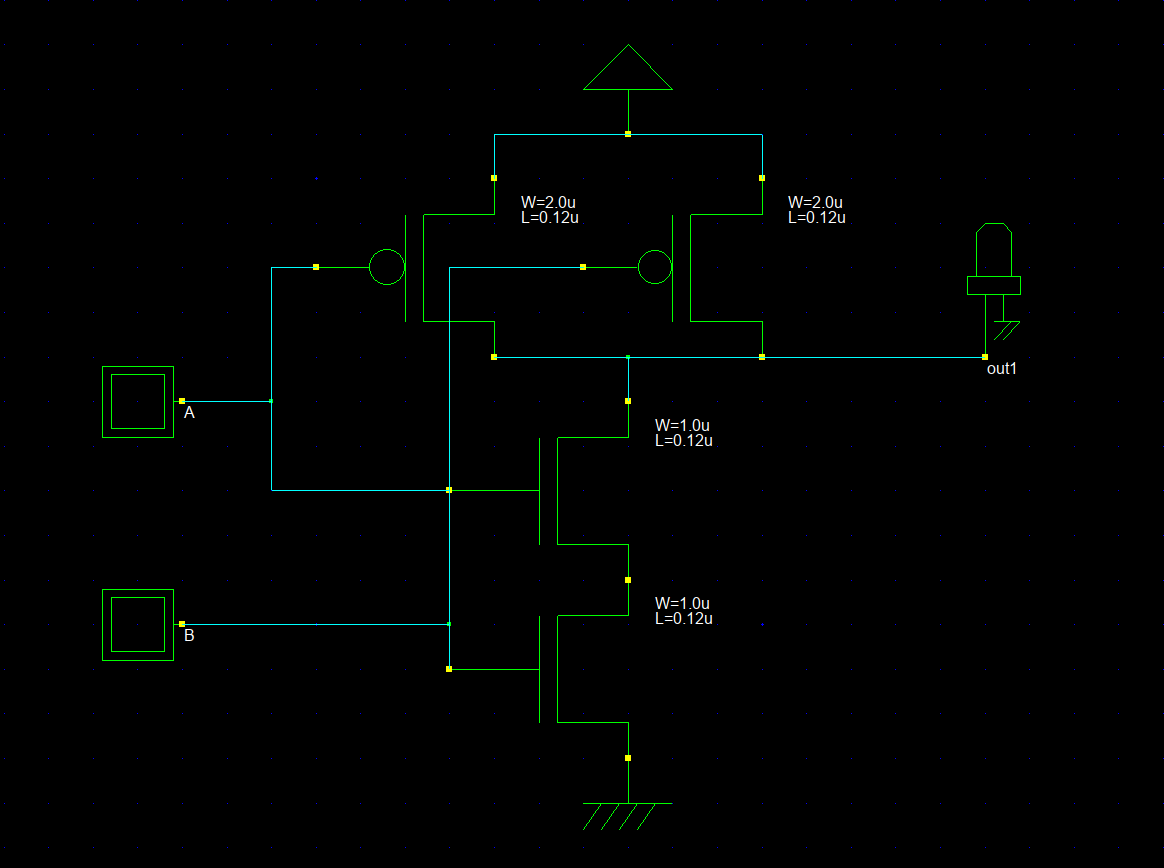
\includegraphics[width=0.8\textwidth]{Lab-01/2in-NAND.png}
    \caption{Schematic of the 2-input NAND}
\end{figure}

\subsection*{Truth Table}
\begin{center}
\begin{tabular}{|c|c|c|}
\hline
A & B & Y \\ \hline
0 & 0 & 1 \\
0 & 1 & 1 \\
1 & 0 & 1 \\
1 & 1 & 0 \\ \hline
\end{tabular}
\end{center}

\subsection*{Observation}
From the simulation results in DSCH2, it was observed that the output of the 2-input NAND gate remains at logic HIGH for all input combinations except when both inputs A and B are logic HIGH. When either input is logic LOW, the output stays HIGH. The output transitions to logic LOW only for the input condition A = 1 and B = 1. These observations are fully consistent with the theoretical truth table of a 2-input NAND gate, confirming correct logical operation of the designed schematic.




\section{3-input NAND}
A 3-input NAND gate outputs a logic LOW only when all three inputs are logic HIGH. For any other input combination, the output remains logic HIGH.

\subsection*{Schematic Image}
\begin{figure}[h!]
    \centering
    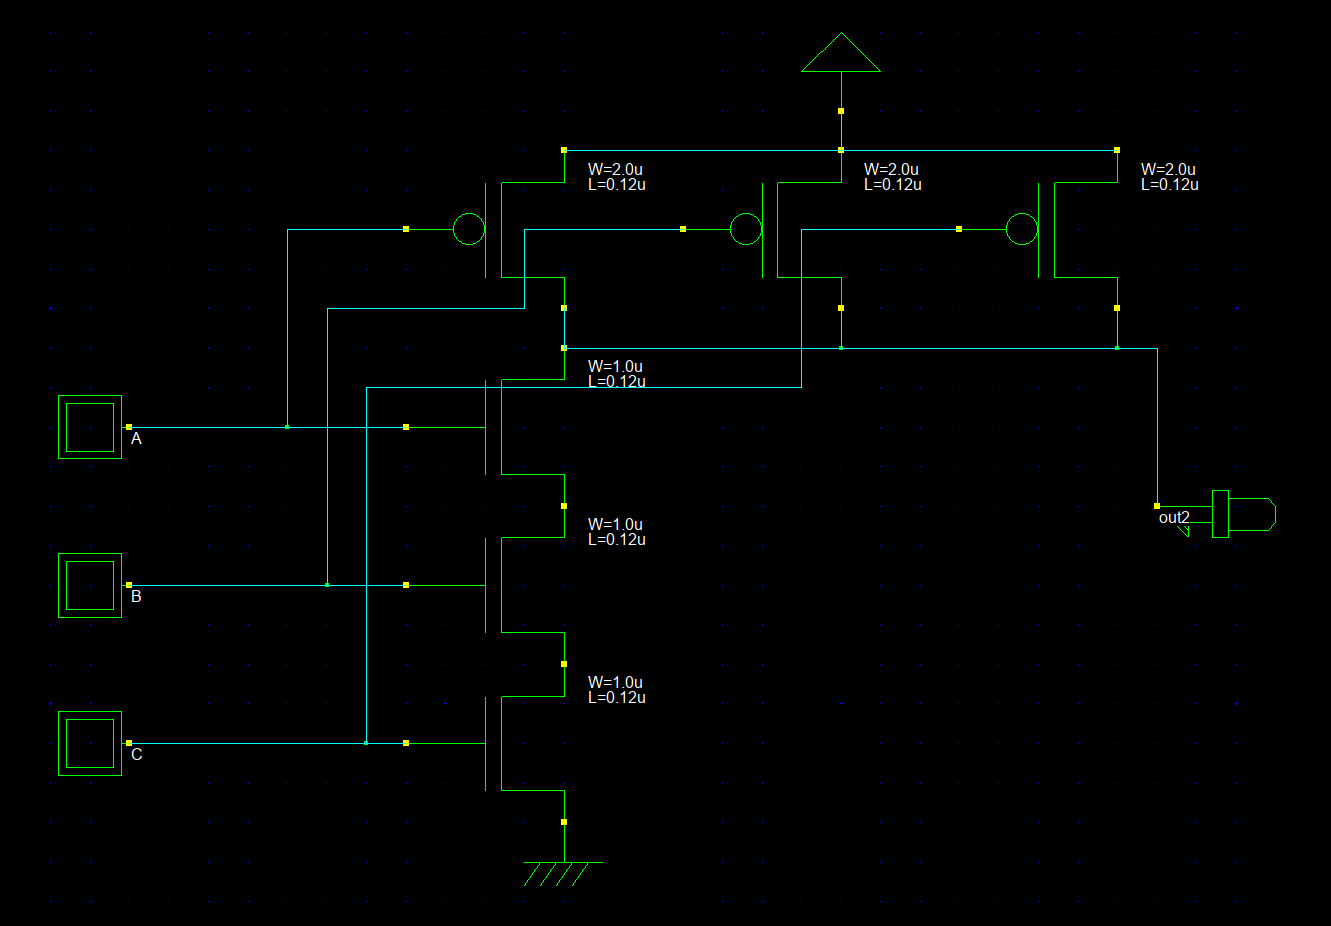
\includegraphics[width=0.7\textwidth]{Lab-01/3in-NAND.png}
    \caption{Schematic of the 3-input NAND}
\end{figure}

\subsection*{Truth Table}
\begin{center}
\begin{tabular}{|c|c|c|c|}
\hline
A & B & C & Y \\ \hline
0 & 0 & 0 & 1 \\
0 & 0 & 1 & 1 \\
0 & 1 & 0 & 1 \\
0 & 1 & 1 & 1 \\
1 & 0 & 0 & 1 \\
1 & 0 & 1 & 1 \\
1 & 1 & 0 & 1 \\
1 & 1 & 1 & 0 \\ \hline
\end{tabular}
\end{center}

\subsection*{Observation}
From the truth table and simulation results, it was observed that the output of the 3-input NAND gate remains at logic HIGH for all input combinations except when all three inputs (A, B, and C) are simultaneously at logic HIGH. In the case where A = 1, B = 1, and C = 1, the output transitions to logic LOW. This behavior confirms that the gate performs the logical negation of the AND operation for three inputs. The observed output values from the DSCH2 simulation precisely matched the theoretical truth table, indicating correct functionality of the 3-input NAND gate.


% ---------------------------------------------------


\section{2-input NOR}
A 2-input NOR gate produces a logic HIGH output only when both inputs are logic LOW. For all other input combinations, the output is logic LOW. NOR gates are also universal gates in digital logic design.

\subsection*{Schematic Image}
\begin{figure}[h!]
    \centering
    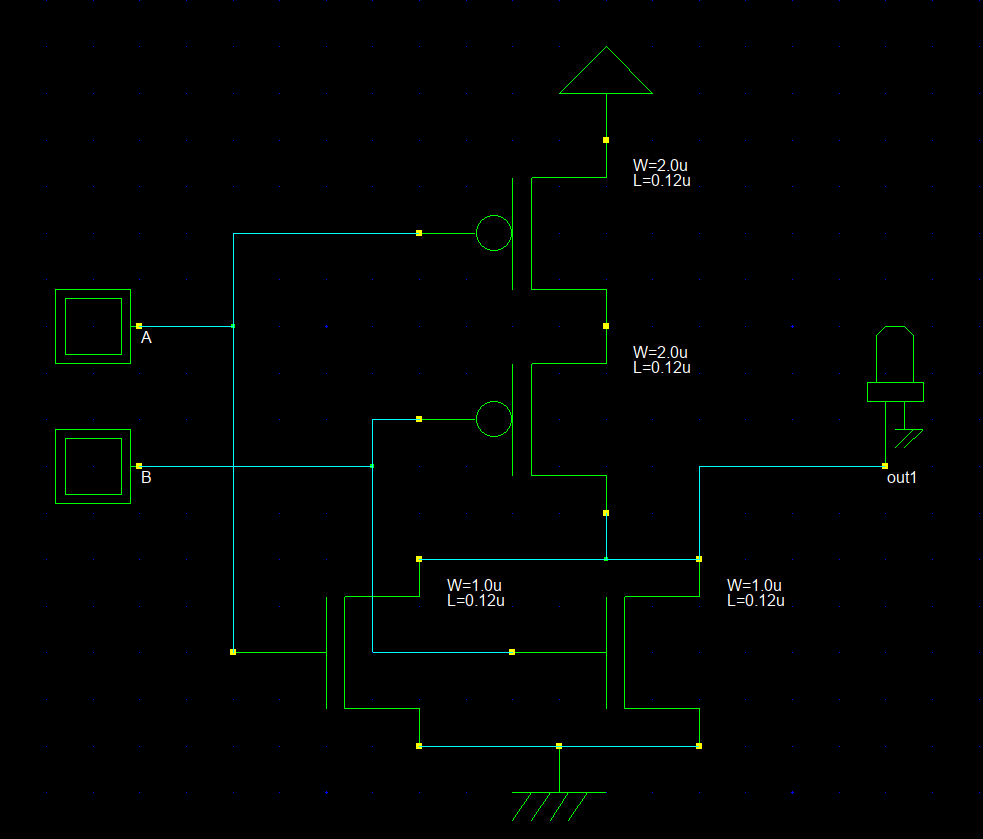
\includegraphics[width=0.8\textwidth]{Lab-01/2in-NOR.png}
    \caption{Schematic of the 2-input NOR}
\end{figure}

\subsection*{Truth Table}
\begin{center}
\begin{tabular}{|c|c|c|}
\hline
A & B & Y \\ \hline
0 & 0 & 1 \\
0 & 1 & 0 \\
1 & 0 & 0 \\
1 & 1 & 0 \\ \hline
\end{tabular}
\end{center}

\subsection*{Observation}
From the truth table and simulation results, it is observed that the output of the 2-input NOR gate remains at logic HIGH only when both inputs A and B are at logic LOW. For all other input combinations where at least one input is logic HIGH, the output transitions to logic LOW. This behavior confirms that the circuit performs the logical NOR operation correctly, as verified through DSCH2 simulation.


% ---------------------------------------------------


\section{3-input NOR}

\subsection*{Schematic Image}
\begin{figure}[h!]
    \centering
    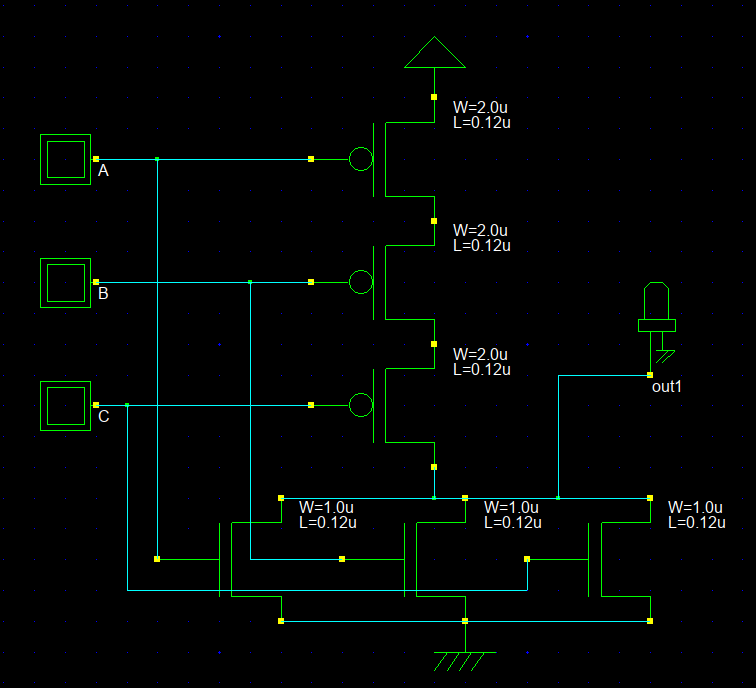
\includegraphics[width=0.65\textwidth]{Lab-01/3in-NOR.png}
    \caption{Schematic of the 3-input NOR}
\end{figure}

\subsection*{Truth Table}
\begin{center}
\begin{tabular}{|c|c|c|c|}
\hline
A & B & C & Y \\ \hline
0 & 0 & 0 & 1 \\
0 & 0 & 1 & 0 \\
0 & 1 & 0 & 0 \\
0 & 1 & 1 & 0 \\
1 & 0 & 0 & 0 \\
1 & 0 & 1 & 0 \\
1 & 1 & 0 & 0 \\
1 & 1 & 1 & 0 \\ \hline
\end{tabular}
\end{center}

\subsection*{Observation}
From the simulation results, it is observed that the output of the 3-input NOR gate becomes logic HIGH only when all three inputs (A, B, and C) are at logic LOW. For any input combination where at least one input is HIGH, the output remains logic LOW. This behavior is consistent with the truth table of the 3-input NOR gate. The DSCH2 simulation output accurately reflects the expected NOR operation, confirming the correctness of the schematic design.


% ---------------------------------------------------


\section{AND Gate}
An AND gate outputs logic HIGH only when all inputs are HIGH.

\subsection*{Schematic Image}
\begin{figure}[h!]
    \centering
    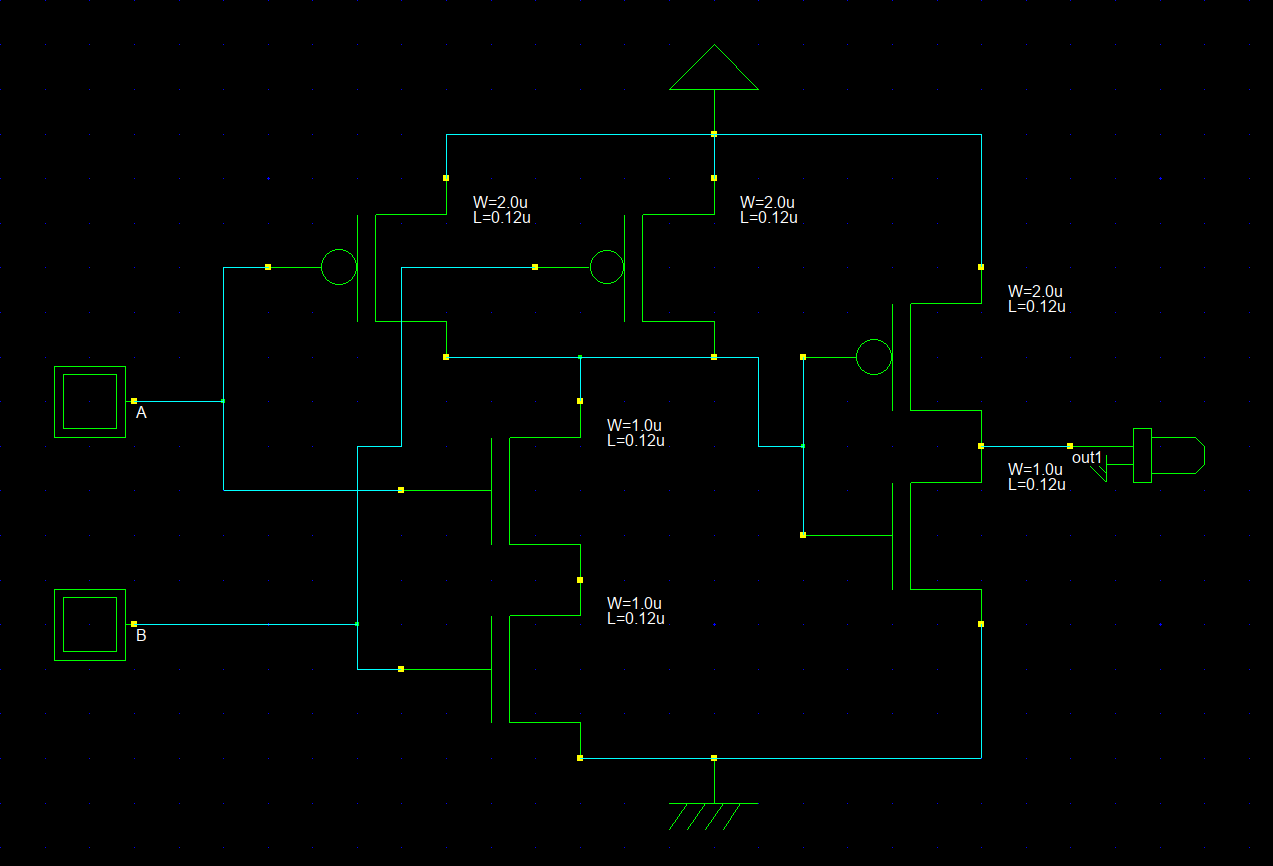
\includegraphics[width=1\textwidth]{Lab-01/2in-AND.png}
    \caption{Schematic of the AND Gate}
\end{figure}

\subsection*{Truth Table}
\begin{center}
\begin{tabular}{|c|c|c|}
\hline
A & B & Y \\ \hline
0 & 0 & 0 \\
0 & 1 & 0 \\
1 & 0 & 0 \\
1 & 1 & 1 \\ \hline
\end{tabular}
\end{center}

\subsection*{Observation}
From the simulation results of the 2-input AND gate in DSCH2, it was observed that the output remains at logic LOW when any one or both of the inputs are at logic LOW. The output transitions to logic HIGH only when both inputs A and B are simultaneously at logic HIGH. This behavior is consistent with the truth table of an AND gate, confirming that the implemented schematic operates correctly.


% ---------------------------------------------------


\section{OR Gate}
An OR gate produces logic HIGH when at least one input is HIGH.

\subsection*{Schematic Image}
\begin{figure}[h!]
    \centering
    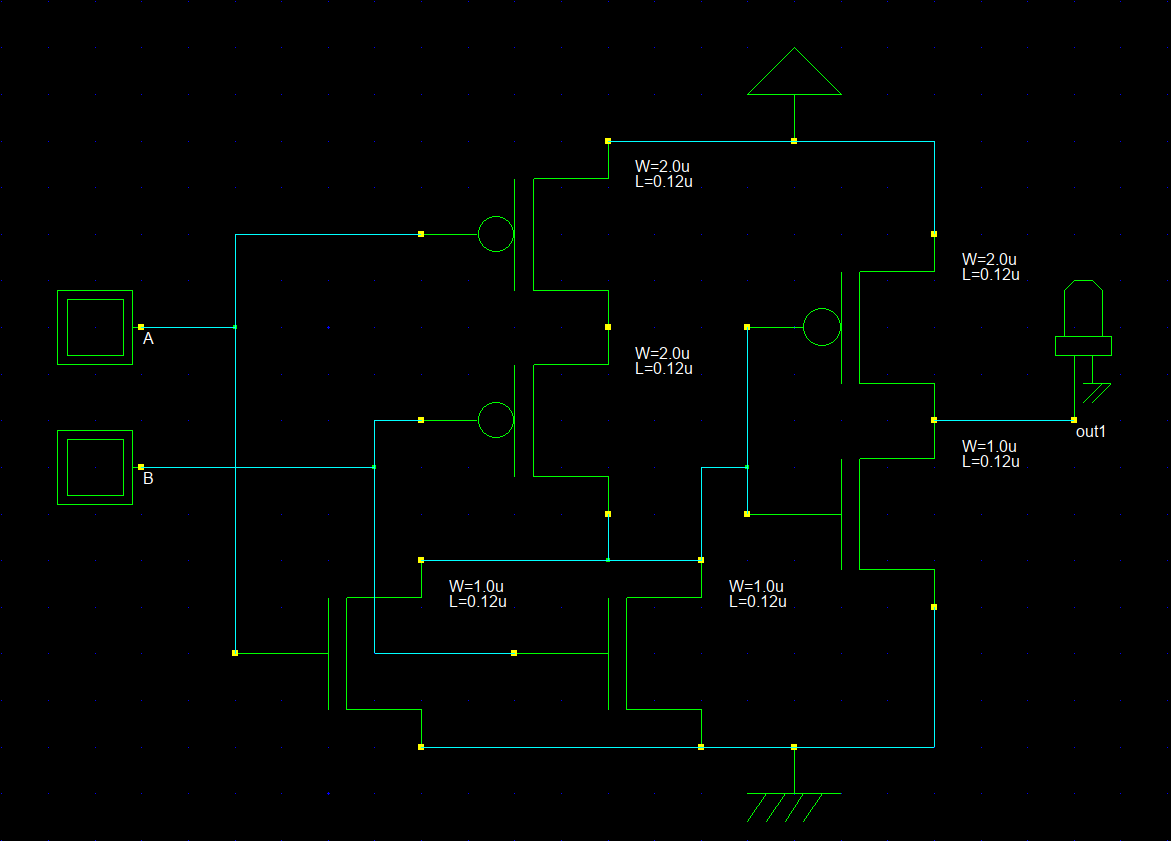
\includegraphics[width=0.9\textwidth]{Lab-01/2in-OR.png}
    \caption{Schematic of the OR Gate}
\end{figure}

\subsection*{Truth Table}
\begin{center}
\begin{tabular}{|c|c|c|}
\hline
A & B & Y \\ \hline
0 & 0 & 0 \\
0 & 1 & 1 \\
1 & 0 & 1 \\
1 & 1 & 1 \\ \hline
\end{tabular}
\end{center}

\subsection*{Observation}
From the simulation results obtained in DSCH2, it was observed that the output of the 2-input OR gate becomes logic HIGH whenever at least one of the inputs is at logic HIGH. When both inputs A and B are at logic LOW, the output remains logic LOW. The simulation output exactly follows the theoretical truth table of the OR gate, confirming that the gate correctly performs the logical OR operation.



% ---------------------------------------------------


\section{XOR Gate}
An XOR gate outputs logic HIGH when the inputs are different.

\subsection*{Schematic Image}
\begin{figure}[h!]
    \centering
    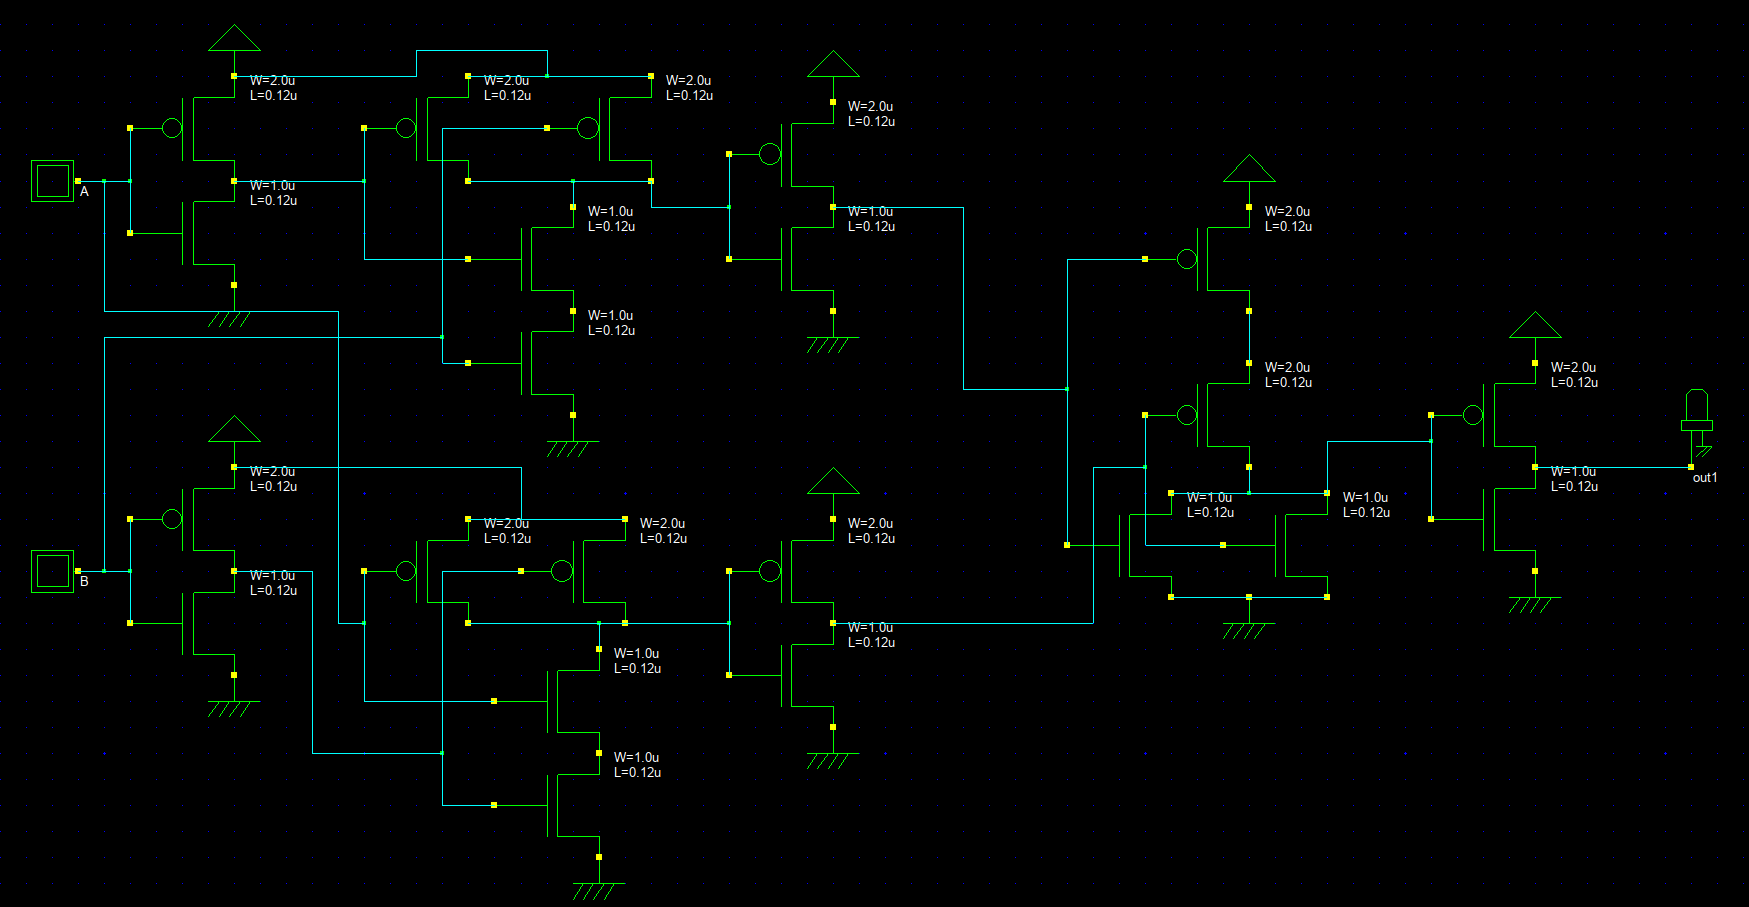
\includegraphics[width=1\textwidth]{Lab-01/2in-XOR.png}
    \caption{Schematic of the XOR Gate}
\end{figure}

\subsection*{Truth Table}
\begin{center}
\begin{tabular}{|c|c|c|}
\hline
A & B & Y \\ \hline
0 & 0 & 0 \\
0 & 1 & 1 \\
1 & 0 & 1 \\
1 & 1 & 0 \\ \hline
\end{tabular}
\end{center}

\subsection*{Observation}
From the simulation results of the 2-input XOR gate in DSCH2, it was observed that the output remains logic LOW when both inputs are at the same logic level, i.e., when both inputs are LOW (0,0) or both inputs are HIGH (1,1). The output becomes logic HIGH when the inputs are different, i.e., for input combinations (0,1) and (1,0). These observations exactly match the theoretical truth table of the XOR gate, confirming that the circuit correctly performs the exclusive-OR operation.





\chapter{Implementing Sequential Circuit}
\lhead{Lab-02: Implementing Sequential Circuit}
\section*{Introduction}
The objective of this laboratory experiment is to implement given Boolean expressions using CMOS logic and verify their functional correctness through schematic design and timing simulation. The circuits were designed using the DSCH2 schematic editor, following standard CMOS pull-up and pull-down network principles. Truth tables and timing diagrams were analyzed to validate logical behavior.


\section*{Objective}
The objectives of this VLSI-Lab experiment are as follows:
\begin{itemize}
    \item To implement given Boolean expressions using CMOS logic design methodology.
    \item To design schematic-level CMOS circuits using the DSCH2 tool.
    \item To verify the logical correctness of the implemented circuits using truth tables.
    \item To analyze timing diagrams to observe signal transitions and propagation behavior.
    \item To develop a clear understanding of CMOS pull-up and pull-down network operation.
\end{itemize}

\section{Function 1: $(ABC + D)'$}

\subsection*{Boolean Function}
\[
Y = (ABC + D)'
\]

\subsection*{Truth Table}
\begin{center}
\begin{tabular}{|c|c|c|c|c|}
\hline 
A & B & C & D & Y \\ \hline
0 & 0 & 0 & 0 & 1 \\
0 & 0 & 1 & 0 & 1 \\
0 & 1 & 0 & 0 & 1 \\
0 & 1 & 1 & 0 & 1 \\
1 & 1 & 1 & 0 & 0 \\
X & X & X & 1 & 0 \\ \hline
\end{tabular}
\end{center}

\subsection*{Schematic Image}
\begin{figure}[!h]
\centering
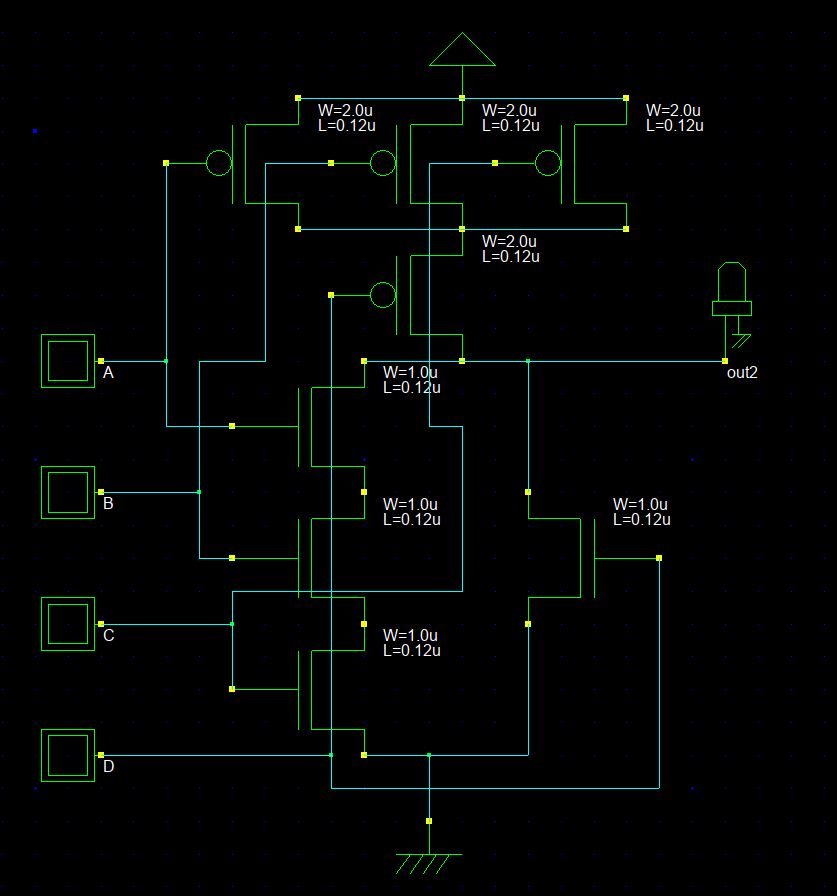
\includegraphics[width=0.5\textwidth]{Lab-02/output-1.png}
\caption{CMOS Schematic of $(ABC + D)'$}
\end{figure}

\subsection*{Timing Diagram}
\begin{figure}[!h]
\centering
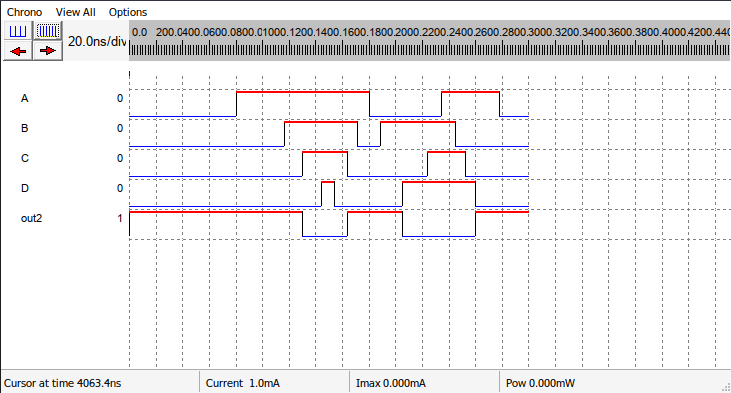
\includegraphics[width=0.7\textwidth]{Lab-02/timing-1.png}
\caption{Timing Diagram of $(ABC + D)'$}
\end{figure}
  
The timing diagram shows that the output remains HIGH except when all inputs A, B, and C are HIGH or when input D is HIGH.

\subsection*{Observation}
The simulation confirms that the output goes LOW when either $ABC=1$ or $D=1$. This matches the expected inverted logic behavior.

% =====================================================
\section{Function 2: $((AB + CD)E)'$}

\subsection*{Boolean Function}
\[
Y = ((AB + CD)E)'
\]

\subsection*{Truth Table}
\begin{center}
\begin{tabular}{|c|c|c|c|c|c|}
\hline
A & B & C & D & E & Y \\ \hline
0 & X & X & X & X & 1 \\
1 & 1 & X & X & 1 & 0 \\
0 & X & 1 & 1 & 1 & 0 \\ 
1 & X & X & X & 1 & 1 \\ \hline
\end{tabular}
\end{center}

\subsection*{Schematic Image}
\begin{figure}[!h]
\centering
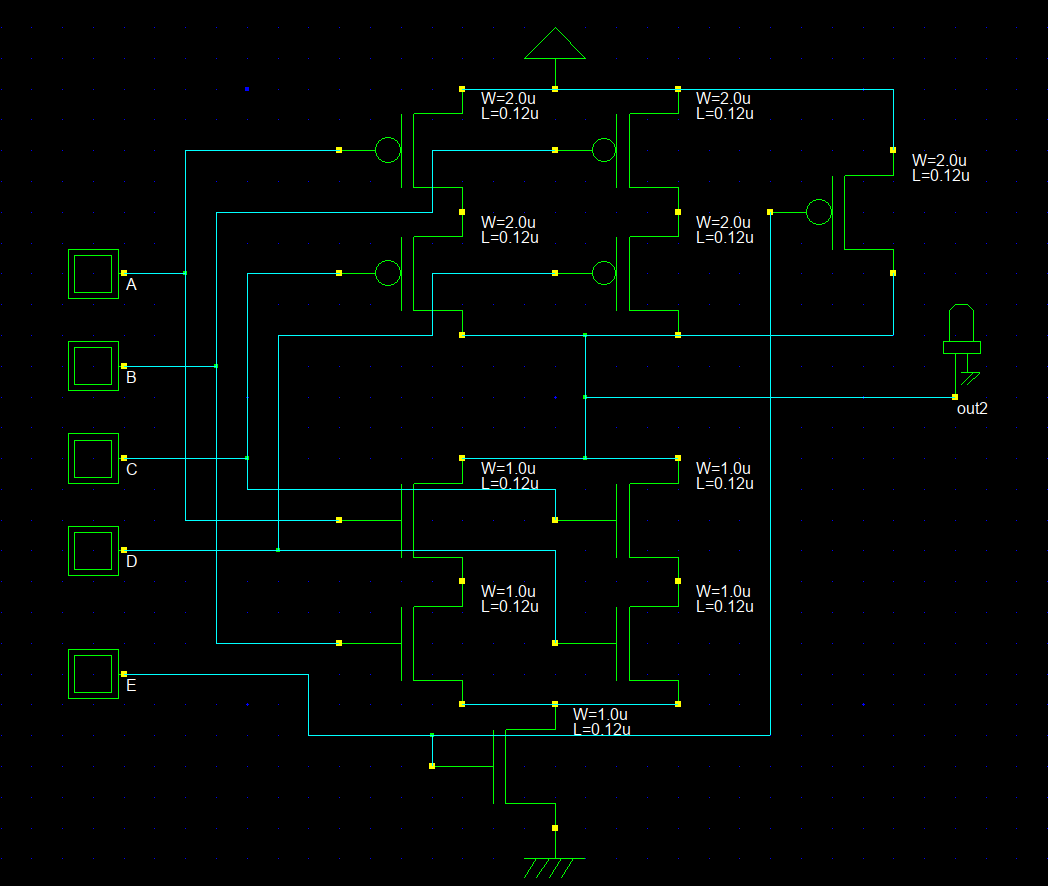
\includegraphics[width=0.9\textwidth]{Lab-02/output-2.png}
\caption{CMOS Schematic of $((AB+CD)E)'$}
\end{figure}
\newpage
\subsection*{Timing Diagram}
\begin{figure}[!h]
\centering
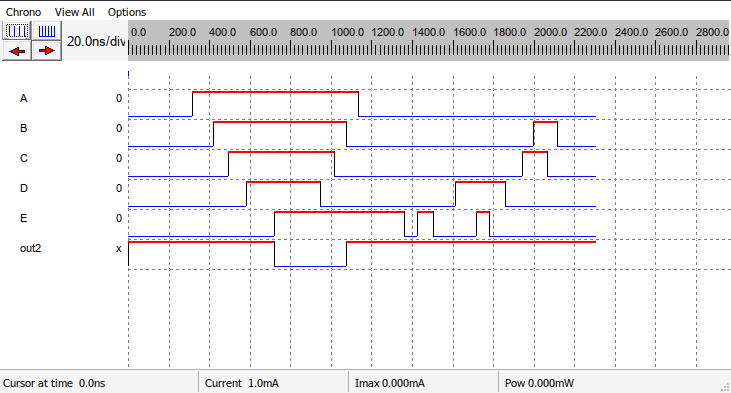
\includegraphics[width=0.9\textwidth]{Lab-02/timing-2.png}
\caption{Timing Diagram of $((AB+CD)E)'$}
\end{figure}

 
The output transitions LOW only when E is HIGH and either AB or CD is satisfied.

\subsection*{Observation}
The circuit output follows the complemented logic, validating correct CMOS pull-up and pull-down network operation.


% =====================================================
\section{Function 3: $((AB + C)(A + B))'$}

\subsection*{Boolean Function}
\[
Y = ((AB + C)(A + B))'
\]

\subsection*{Truth Table}
\begin{center}
\begin{tabular}{|c|c|c|c|}
\hline
A & B & C & Y \\ \hline
0 & 0 & 0 & 1 \\
0 & 1 & 0 & 1 \\
1 & 0 & 0 & 1 \\
1 & 1 & 0 & 0 \\
1 & 0 & 1 & 0 \\ 
1 & 1 & 1 & 0 \\ \hline
\end{tabular}
\end{center}
\newpage
\subsection*{Schematic Image}
\begin{figure}[!h]
\centering
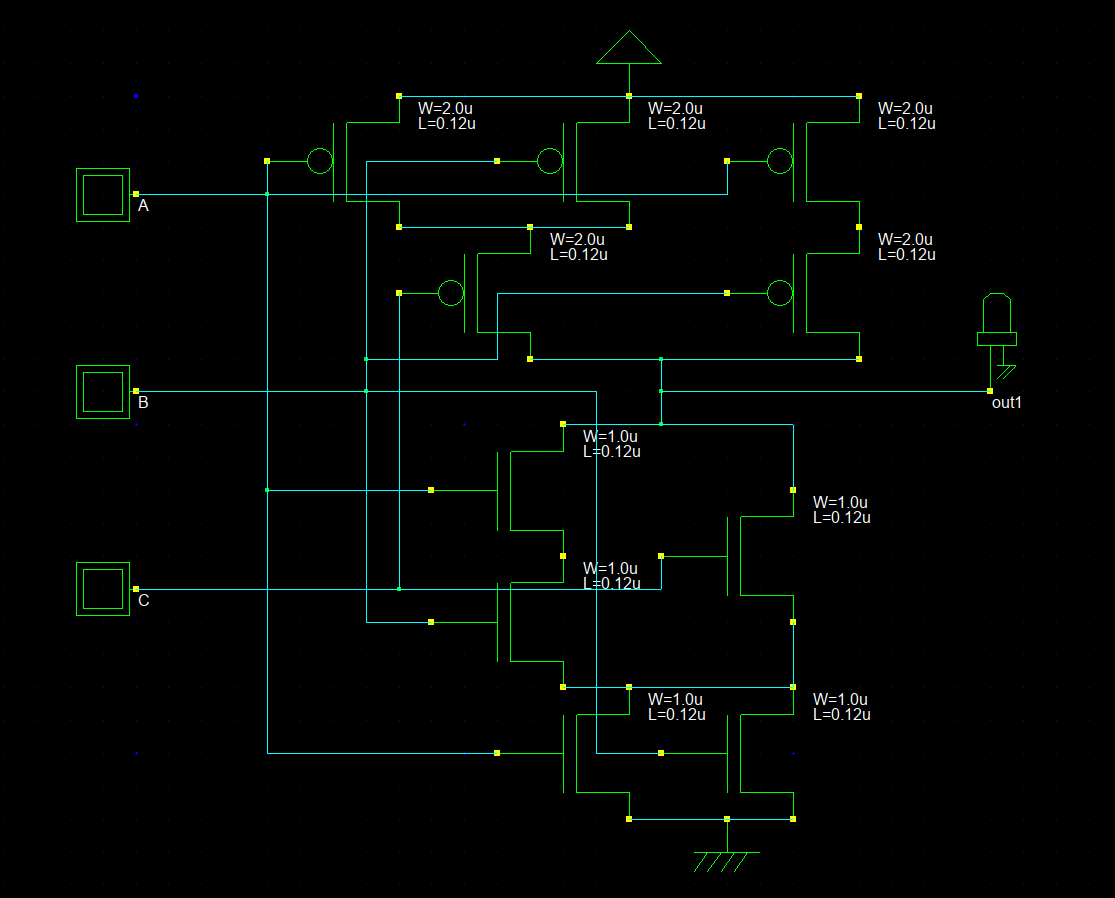
\includegraphics[width=0.8\textwidth]{Lab-02/output-3.png}
\caption{CMOS Schematic of $((AB + C)(A + B))'$}
\end{figure}

\subsection*{Timing Diagram}
\begin{figure}[!h]
\centering
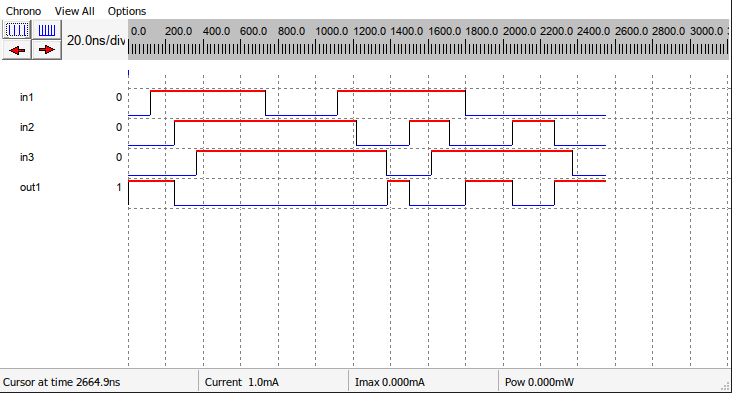
\includegraphics[width=0.8\textwidth]{Lab-02/timing-3.png}
\caption{Timing Diagram of $((AB + C)(A + B))'$}
\end{figure}

 
The output remains HIGH only when the AND of the two expressions is false.

\subsection*{Observation}
Simulation results matched the inverted product-of-sums logic expression.


% =====================================================
\section{Function 4: $(A + B + C)D$}

\subsection*{Boolean Function}
\[
Y = (A + B + C)D
\]

\subsection*{Truth Table}
\begin{center}
\begin{tabular}{|c|c|c|c|c|}
\hline
A & B & C & D & Y \\ \hline
X & X & X & 0 & 0 \\
1 & X & X & 1 & 1 \\
0 & 1 & X & 1 & 1 \\
0 & 0 & 1 & 1 & 1 \\
0 & 0 & 0 & 1 & 0 \\ \hline
\end{tabular}
\end{center}

\subsection*{Schematic Image}
\begin{figure}[!h]
\centering
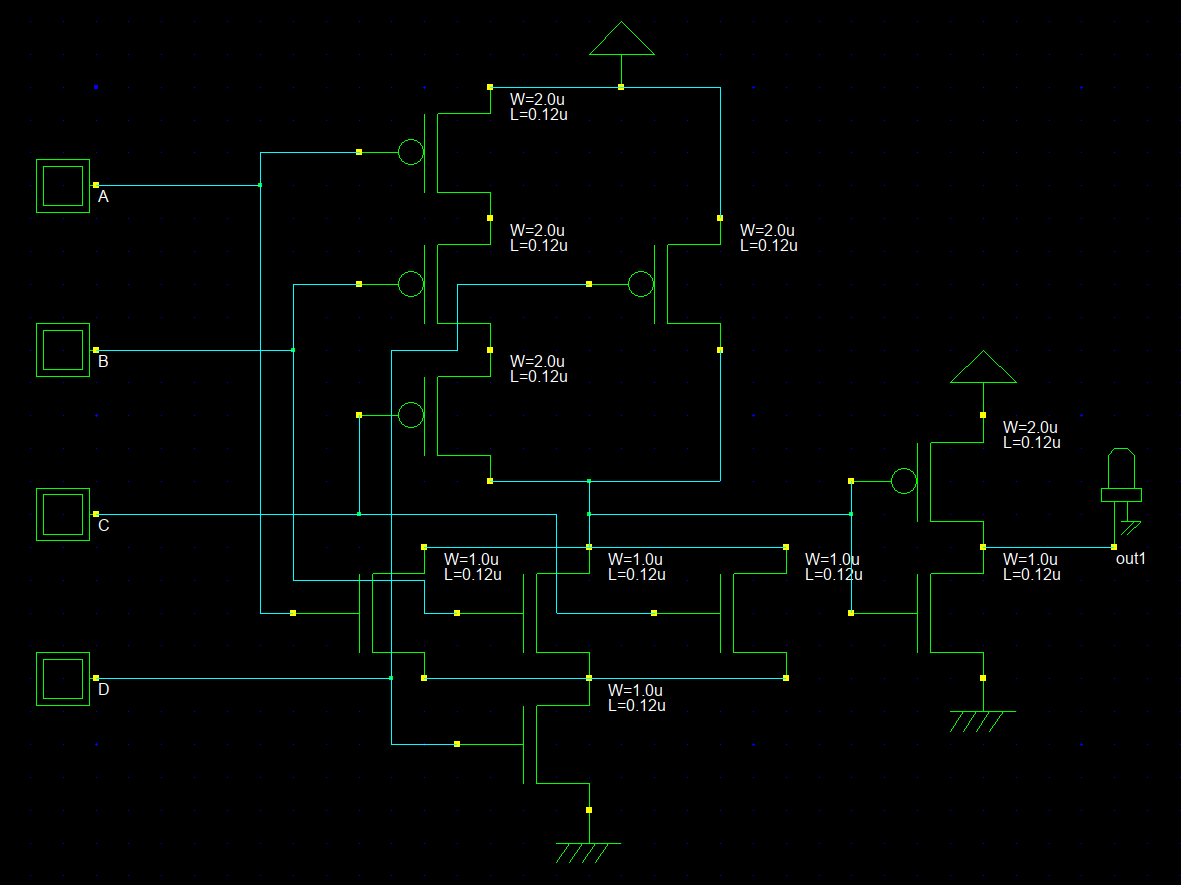
\includegraphics[width=0.9\textwidth]{Lab-02/output-4.png}
\caption{CMOS Schematic of $(A+B+C)D$}
\end{figure}
\newpage
\subsection*{Timing Diagram}
\begin{figure}[!h]
\centering
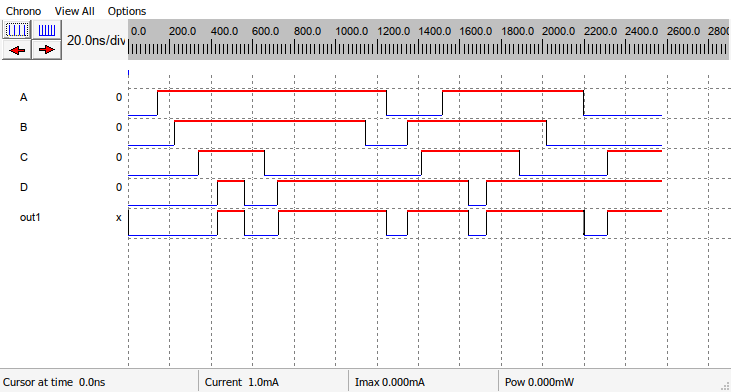
\includegraphics[width=0.9\textwidth]{Lab-02/timing-4.png}
\caption{Timing Diagram of $(A+B+C)D$}
\end{figure}
 
The output is HIGH only when D is HIGH and at least one of A, B, or C is HIGH.

\subsection*{Observation}
The simulation confirms correct AND–OR logic behavior.


% =====================================================
\section{Function 5: $((A + B)CD)'$}

\subsection*{Boolean Function}
\[
Y = ((A + B)CD)'
\]

\subsection*{Truth Table}
\begin{center}
\begin{tabular}{|c|c|c|c|c|}
\hline
A & B & C & D & Y \\ \hline
X & X & X & 0 & 1 \\
0 & 0 & 1 & 1 & 1 \\
1 & X & 1 & 1 & 0 \\
X & 1 & 1 & 1 & 0 \\ \hline
\end{tabular}
\end{center}
\newpage
\subsection*{Schematic Image}
\begin{figure}[!h]
\centering
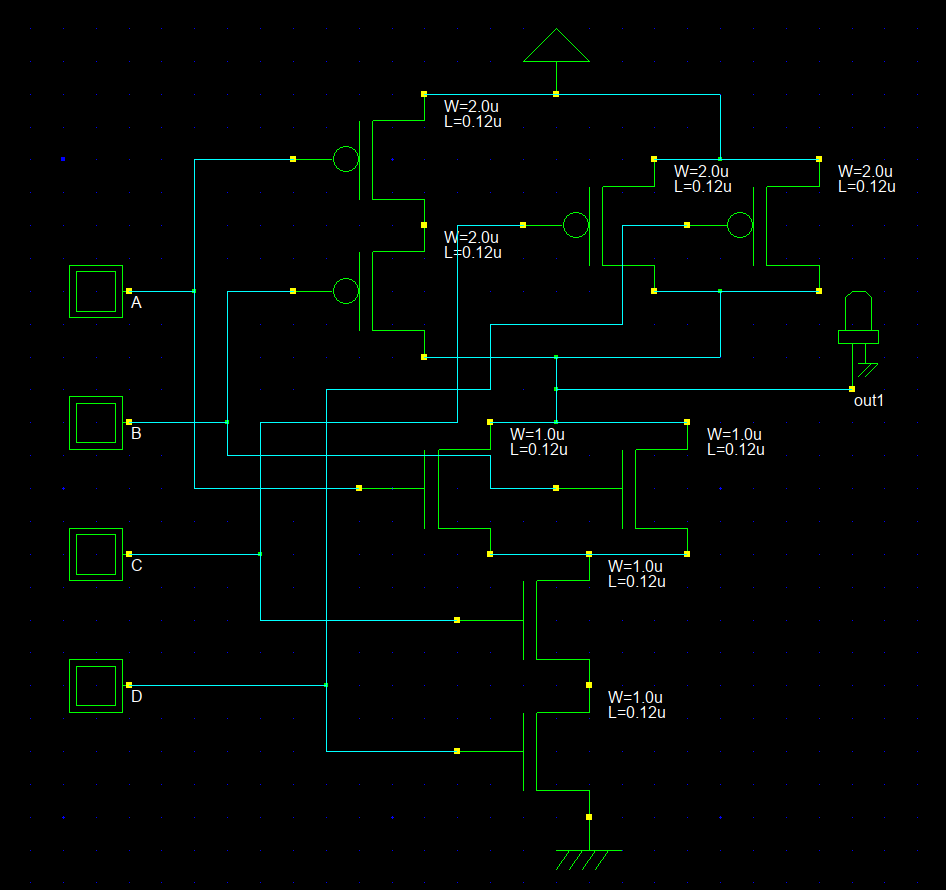
\includegraphics[width=0.6\textwidth]{Lab-02/output-5.png}
\caption{CMOS Schematic of $((A+B)CD)'$}
\end{figure}

\subsection*{Timing Diagram}
\begin{figure}[!h]
\centering
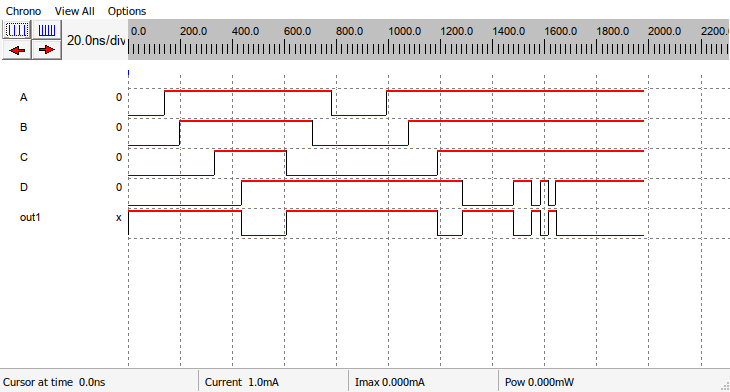
\includegraphics[width=0.8\textwidth]{Lab-02/timing-5.png}
\caption{Timing Diagram of $((A+B)CD)'$}
\end{figure}

\subsection*{Observation} 
The output goes LOW only when C and D are HIGH and either A or B is HIGH.
Simulation results confirm correct inverted AND–OR CMOS implementation.

% =====================================================






\chapter{Adder Circuits}
\lhead{Lab-03: Adder Circuits}

\section*{Introduction}
A combinational logic circuit which is designed to add two binary digits is called as a half adder. The half adder provides the output along with a carry value (if any). The half adder circuit is designed by connecting an EX-OR gate and one AND gate. It has two input terminals and two output terminals for sum and carry.


\section*{Objective}
The objectives of this VLSI-Lab experiment are as follows:
\begin{itemize}
    \item To implement Adder Circuit using CMOS logic design methodology.
    \item To design schematic-level Adder circuits using the DSCH2 tool.
    \item To verify the logical correctness of the implemented circuits using truth tables.
    \item To analyze timing diagrams to observe signal transitions and propagation behavior.
    \item To develop a clear understanding of Adder Circuit.
\end{itemize}

\section{Half Adder Function}

\subsection*{Boolean Function}
\[
Sum = AB' + A'B
\]
\[
Carry= A⋅B
\]

\subsection*{Truth Table}
\begin{center}
\begin{tabular}{|c|c|c|c|c|}
\hline 
A & B & Sum & Carry \\ \hline
0 & 0 & 0 & 0  \\
0 & 1 & 1 & 0  \\
1 & 0 & 1 & 0  \\
1 & 1 & 0 & 1  \\ \hline
\end{tabular}
\end{center}
\newpage
\subsection*{Schematic Image}

\begin{figure}[!h]
\centering
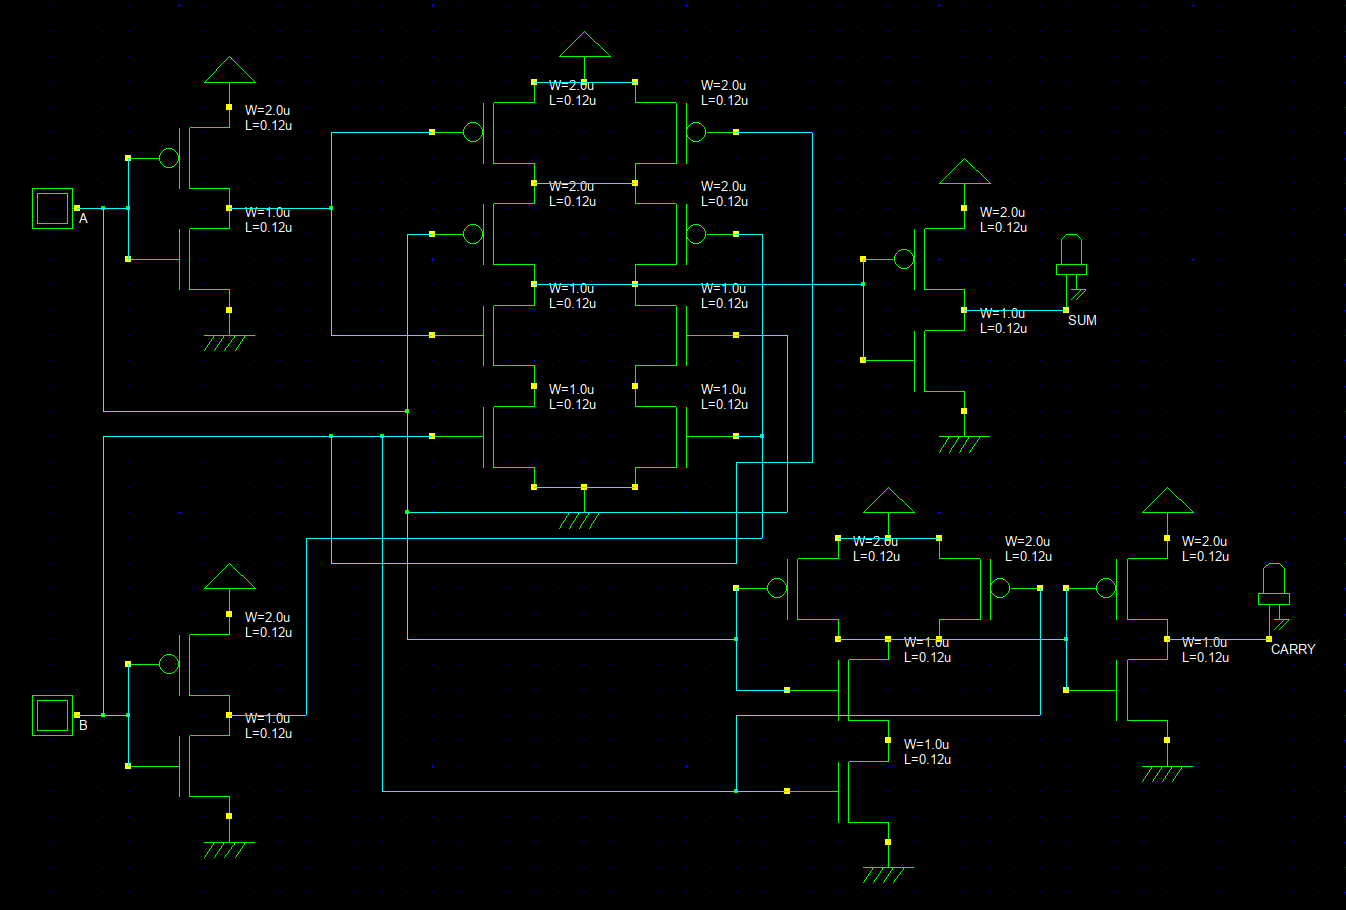
\includegraphics[width=0.7\textwidth]{Lab-03/Half-Adder.png}
\caption{CMOS Schematic of Half-Adder}
\end{figure}

\subsection*{Timing Diagram}
\begin{figure}[!h]
\centering
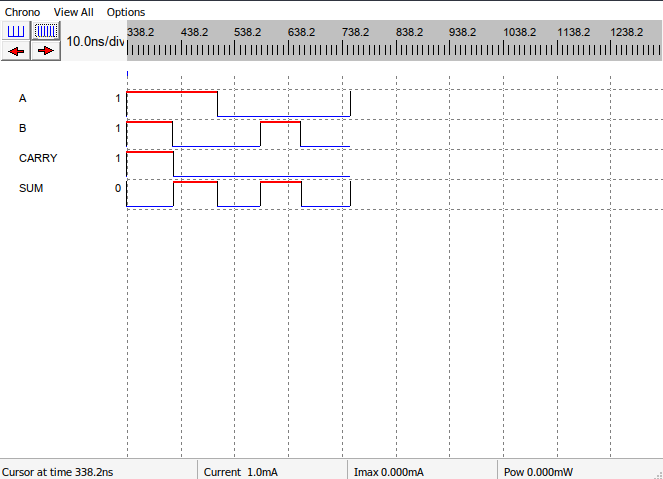
\includegraphics[width=0.5\textwidth]{Lab-03/Half-Adder-TD.png}
\caption{Timing Diagram of Half-Adder}
\end{figure}
  


\subsection*{Observation}
The timing diagram of a half adder illustrates the sequence of operations that occur when two binary inputs are added. The diagram typically shows the timing of the XOR operation for the sum and the timing of the AND operation for the carry. The timing diagram can help in understanding the propagation delay and the timing constraints of the circuit. It is important to note that the timing diagram should be adjusted to account for the specific timing requirements of the circuit design, such as rise/fall time and maximum input frequency. 




\chapter{Flip-Flop Circuits}
\lhead{Lab-04: Flip-Flop Circuits}
\section*{Introduction}
This laboratory experiment focuses on the design and implementation of a flip-flop circuit using CMOS logic in the DSCH2 environment. Flip-flops are fundamental sequential elements used for data storage and synchronization in digital systems. In this experiment, a D Flip-Flop was designed using CMOS-based logic gates, and its functionality was verified through truth table analysis and timing simulation. The behavior of the circuit was observed with respect to clock-triggered input transitions.

\section*{Objective}
The objectives of this laboratory experiment are as follows:
\begin{itemize}
    \item To design and implement a flip-flop circuit using CMOS logic.
    \item To develop schematic-level circuits using the DSCH2 tool.
    \item To derive and verify the truth table of the flip-flop from simulation.
    \item To analyze timing diagrams to observe clock-triggered behavior.
    \item To understand the operation of sequential circuits and data storage elements.
\end{itemize}

\section{Function of FlipFlop Circuit}
The D Flip-Flop is a clock-controlled bistable device that transfers the input data (D) to the output (Q) on the active edge of the clock signal.

\[
Q_{next} = D
\]

The output changes only at the triggering edge of the clock, ensuring synchronized data storage.


\subsection*{Truth Table}
\begin{center}
\begin{tabular}{|c|c|c|}
\hline
Clock & D & Q(next) \\ \hline
$\uparrow$ & 0 & 0 \\
$\uparrow$ & 1 & 1 \\
No Edge & X & Q(previous) \\ \hline
\end{tabular}
\end{center}

\subsection*{Schematic Image}
\begin{figure}[!h]
\centering
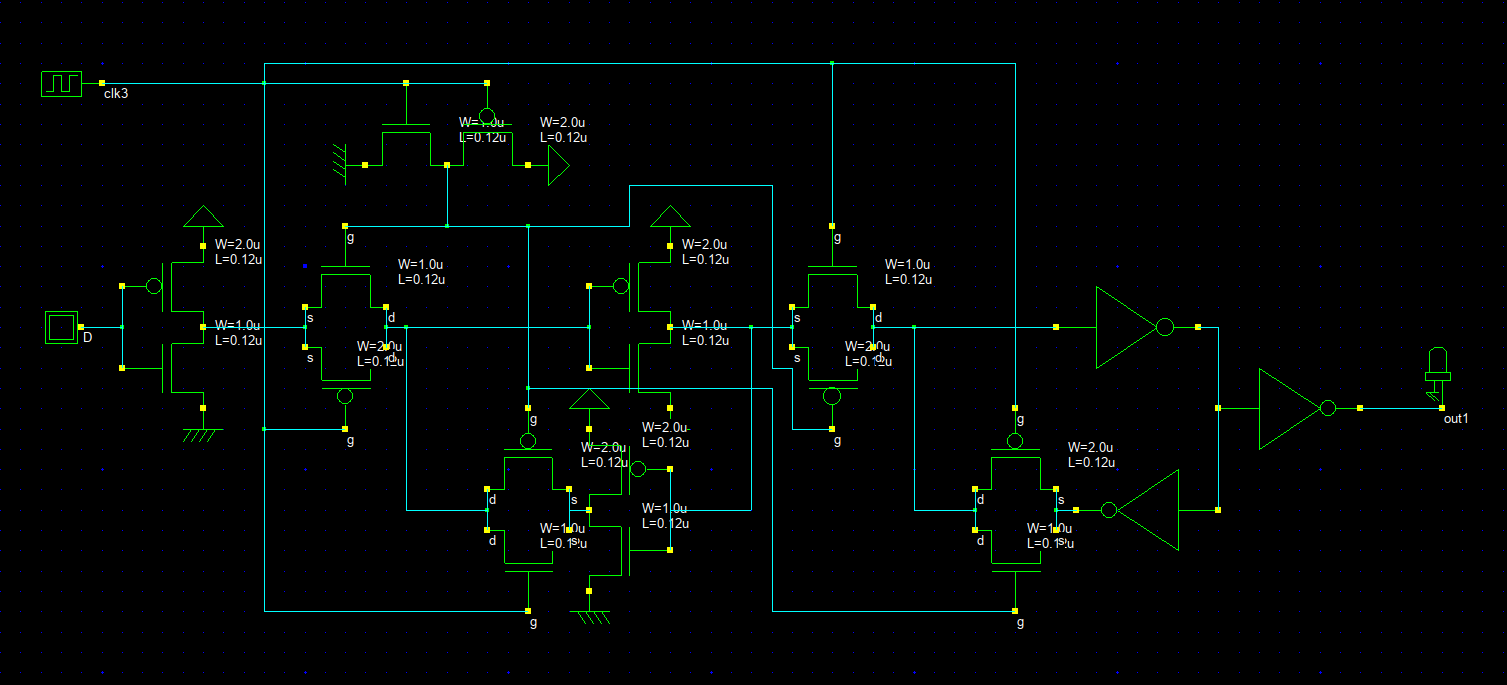
\includegraphics[width=1\textwidth]{Lab-04/FlipFlop.png}
\caption{CMOS Schematic of D Flip-Flop in DSCH2}
\end{figure}


\subsection*{Timing Diagram}
\begin{figure}[!h]
\centering
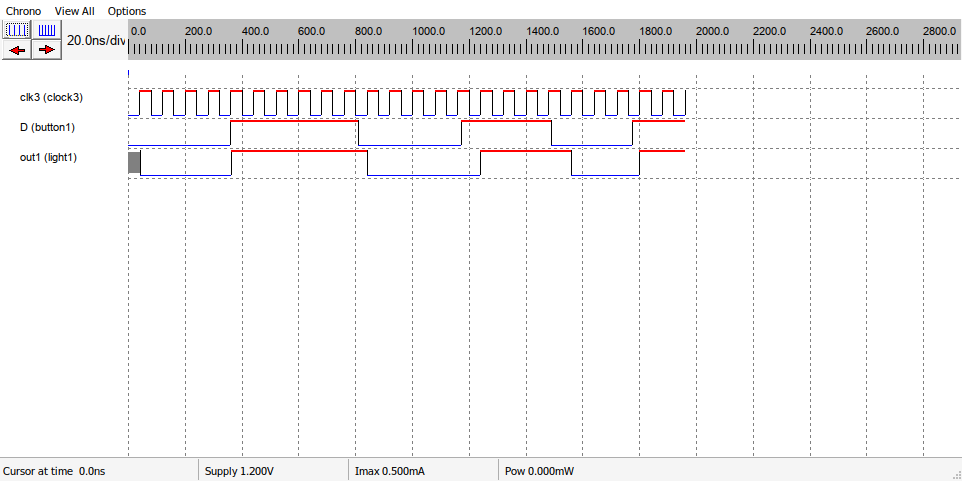
\includegraphics[width=0.7\textwidth]{Lab-04/Timing Diagram.png}
\caption{Timing Diagram of D Flip-Flop}
\end{figure}

\subsection*{Observation}
The timing diagram shows that the output Q follows the input D only at the rising edge of the clock signal. Between clock edges, the output remains constant regardless of changes in the input. \\
From the simulation results, it was observed that the D Flip-Flop changes its output state only at the rising edge of the clock signal. When the clock transitions from LOW to HIGH, the output Q takes the value of the input D. At all other times, the output remains unchanged, preserving the previously stored value. This behavior confirms the correct operation of the edge-triggered D Flip-Flop implemented using CMOS logic.




\chapter{Stick Diagram in MICROWIND2}
\lhead{Lab-05: Stick Diagram in MICROWIND2}

\section*{Introduction}
In VLSI design, the transition from schematic-level representation to physical layout is a critical step in the design process. Stick diagrams serve as an intermediate abstraction that simplifies the visualization of circuit layouts without considering exact dimensions. These diagrams use standardized color codes to represent different layers such as polysilicon, diffusion regions, and metal interconnections.

Microwind2 is a layout design tool that allows designers to implement and simulate CMOS circuits at the physical level. In this experiment, stick diagrams of basic logic gates were implemented to understand layout organization, transistor placement, and interconnection strategies. The study of stick diagrams helps in developing an understanding of design rules, layout optimization, and area-efficient circuit implementation in VLSI systems.


\section*{Objective}
The objectives of this laboratory experiment are as follows:
\begin{itemize}
    \item To understand the concept and importance of stick diagrams in VLSI layout design.
    \item To implement stick diagrams of basic CMOS logic gates using Microwind2.
    \item To represent transistor-level circuits using simplified, technology-independent layouts.
    \item To analyze the arrangement of polysilicon, diffusion, and metal layers in CMOS design.
    \item To develop a clear understanding of the relationship between schematic design and physical layout.
\end{itemize}


\newpage
\section{1 Input Inverter (NOT Gate)}
The inverter, also known as a NOT gate, is the most fundamental logic gate in digital design. It produces the logical complement of the input signal. In CMOS technology, the inverter is implemented using one PMOS transistor in the pull-up network and one NMOS transistor in the pull-down network. The stick diagram represents this structure using polysilicon for gate control, diffusion regions for source and drain, and metal layers for interconnections. The inverter serves as the basic building block for more complex CMOS circuits.

\subsection*{Stick Diagram}
\begin{figure}[!h]
\centering
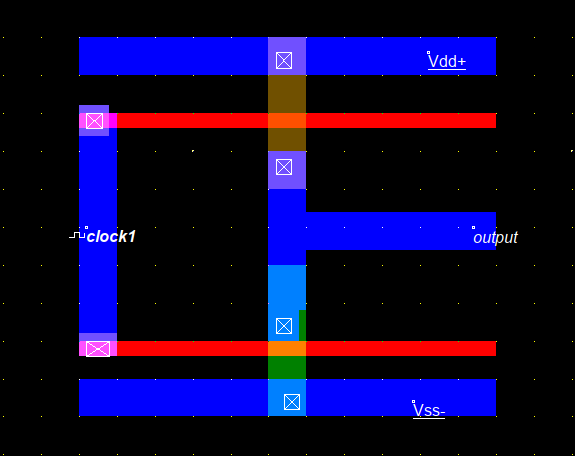
\includegraphics[width=1\textwidth]{Lab-05/Inverter.png}
\caption{Stick Diagram of Inverter (NOT Gate) in MICROWIND2}
\end{figure}
\newpage
\subsection*{Output}
\begin{figure}[!h]
\centering
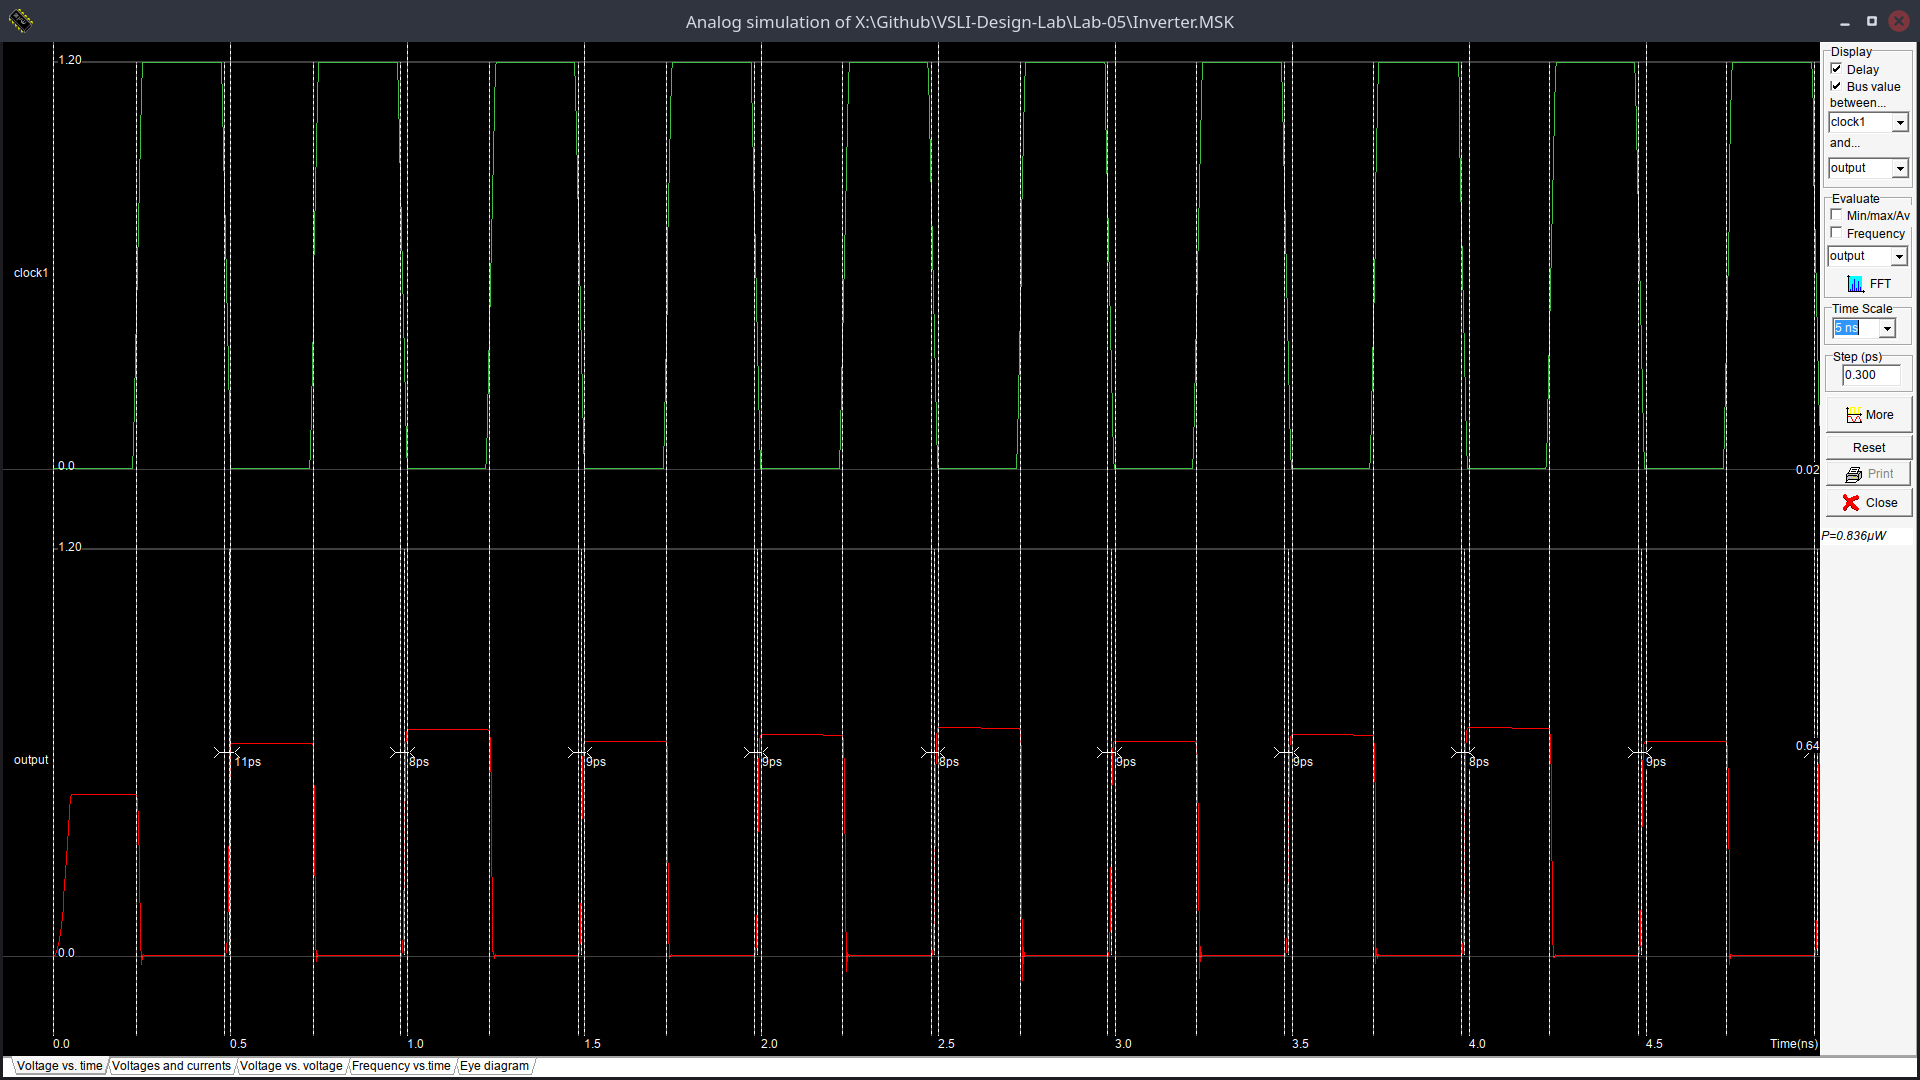
\includegraphics[width=1\textwidth]{Lab-05/Inverter-Out.png}
\caption{Analog Simulation of Inverter (NOT Gate)}
\end{figure}
\subsection*{Observation}
From the output waveform, it is observed that the inverter produces the exact complement of the input signal. When the input is at logic HIGH, the NMOS transistor conducts and pulls the output to logic LOW. Conversely, when the input is at logic LOW, the PMOS transistor conducts and pulls the output to logic HIGH. The transition between output states occurs immediately following the input change, demonstrating correct switching behavior. The observed output confirms the proper operation of the CMOS inverter as expected from its theoretical truth table.





\newpage
\section{2 Input NAND Gate}
A 2-input NAND gate is a fundamental universal logic gate that produces a logic LOW output only when both inputs are logic HIGH. In CMOS layout design, the NAND gate is implemented using two NMOS transistors connected in series in the pull-down network and two PMOS transistors connected in parallel in the pull-up network. The stick diagram represents this structure using simplified layer representations such as polysilicon for gates, diffusion for active regions, and metal for interconnections.

\subsection*{Stick Diagram}
\begin{figure}[!h]
\centering

\includegraphics[width=1\textwidth]{Lab-05/2in-NAND.png}
\caption{Stick Diagram of 2in-NAND Gate in MICROWIND2}
\end{figure}
\newpage
\subsection*{Output}
\begin{figure}[!h]
\centering
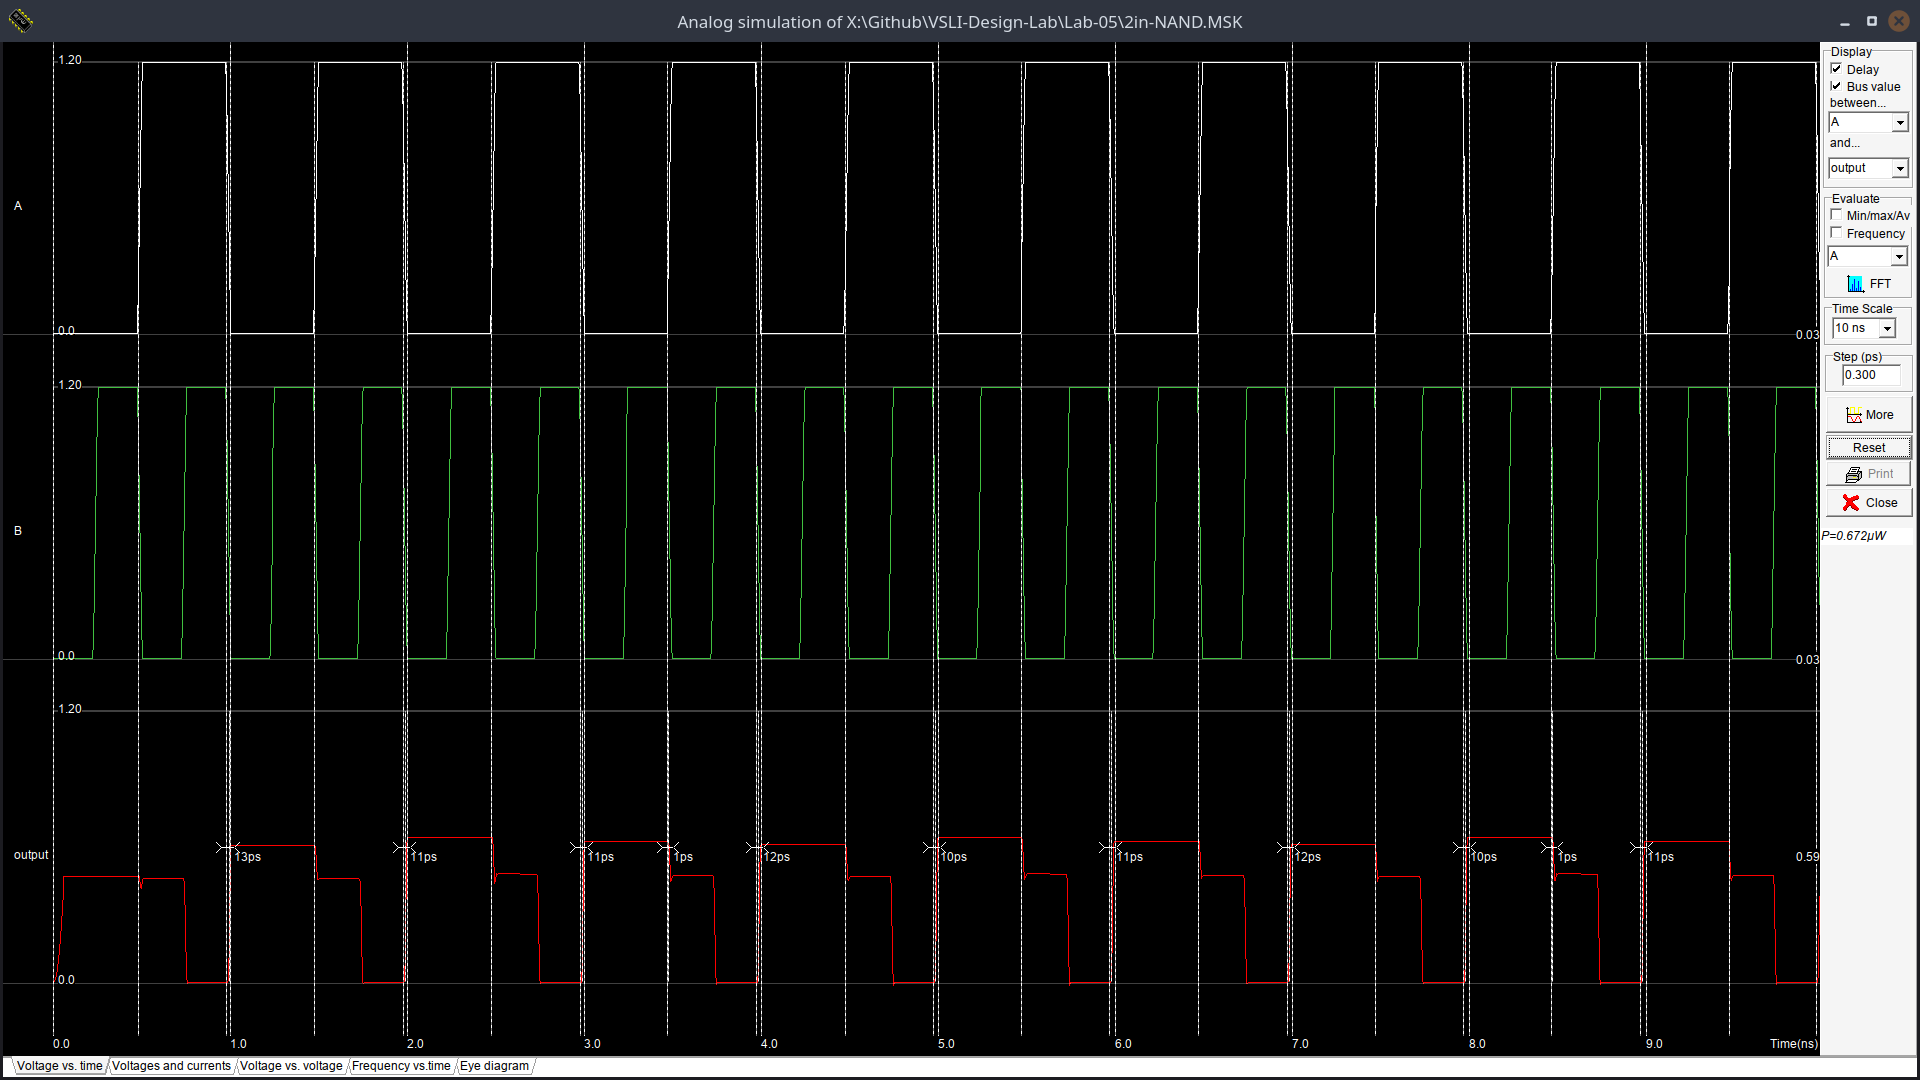
\includegraphics[width=1\textwidth]{Lab-05/2in-NAND-Out.png}
\caption{Analog Simulation of 2in-NAND Gate}
\end{figure}

\subsection*{Observation}
From the simulation results obtained in Microwind2, it is observed that the output remains at logic HIGH for all input combinations except when both inputs are HIGH. When inputs A and B are simultaneously at logic HIGH, the series NMOS transistors in the pull-down network conduct, creating a path to ground and forcing the output to logic LOW. For all other input conditions, at least one PMOS transistor in the pull-up network remains active, maintaining the output at logic HIGH. The observed output waveform matches the expected truth table of a 2-input NAND gate, confirming the correctness of the stick diagram implementation.





\newpage
\section{2 Input NOR Gate}
The 2-input NOR gate is a fundamental digital logic gate that produces a logic HIGH output only when both inputs are at logic LOW. In CMOS implementation, the NOR gate is realized using parallel NMOS transistors in the pull-down network and series PMOS transistors in the pull-up network. In the stick diagram representation using Microwind2, different layers such as polysilicon, diffusion, and metal are arranged according to standard layout conventions to form the required transistor connections. The stick diagram provides a simplified visualization of the physical layout without considering exact dimensions.
\subsection*{Stick Diagram}
\begin{figure}[!h]
\centering

\includegraphics[width=1\textwidth]{Lab-05/2in-NOR.png}
\caption{Stick Diagram of 2in-NOR Gate in MICROWIND2}
\end{figure}
\newpage
\subsection*{Output}
\begin{figure}[!h]
\centering
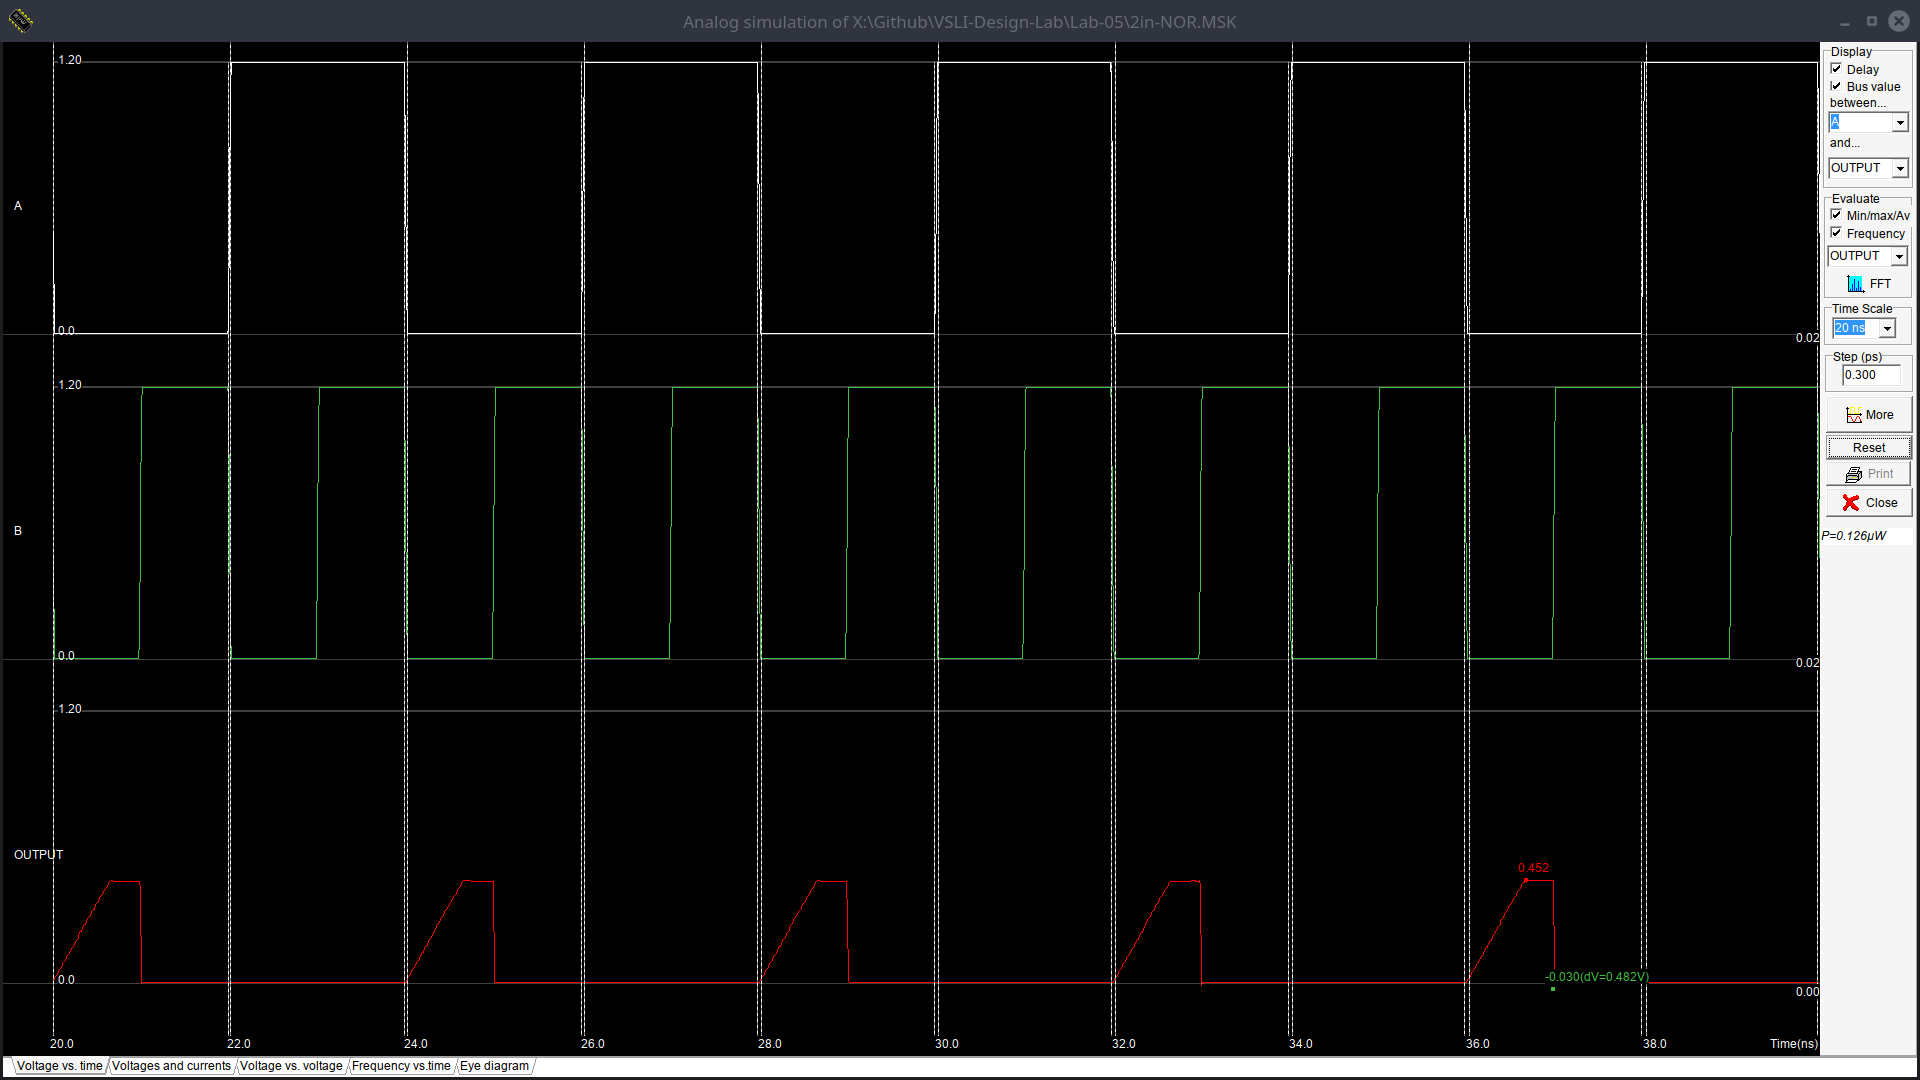
\includegraphics[width=1\textwidth]{Lab-05/2in-NOR-Out.png}
\caption{Analog Simulation of 2in-NOR Gate}
\end{figure}

\subsection*{Observation}
From the simulation results, it is observed that the output of the 2-input NOR gate remains logic HIGH only when both inputs are LOW (0,0). For all other input combinations, i.e., when any one or both inputs are HIGH, the output becomes logic LOW. The output waveform clearly reflects this behavior, showing a HIGH level only in the absence of input signals. This verifies the correct implementation of the NOR logic function in the stick diagram using Microwind2.






\chapter{Stick Diagram of XOR function}
\lhead{Lab-06: Stick Diagram of XOR function}

\section*{Introduction}
In VLSI design, the transformation of logical circuits into physical layouts is an essential step in the design process. Stick diagrams serve as a simplified and technology-independent method for representing circuit layouts, allowing designers to visualize transistor placement and interconnections without focusing on exact dimensions.

The XOR gate is an important combinational logic circuit widely used in arithmetic and digital systems. Its implementation in CMOS requires careful arrangement of pull-up and pull-down networks. In this experiment, the XOR gate is designed using its Boolean expression and represented using a stick diagram in Microwind2. The study of this design helps in understanding layout organization, layer interaction, and efficient circuit realization in VLSI systems.



\section*{Objective}
The objectives of this laboratory experiment are as follows:
\begin{itemize}
    \item To understand the concept and importance of stick diagrams in VLSI layout design.
    \item To implement stick diagrams of basic CMOS logic gates using Microwind2.
    \item To represent transistor-level circuits using simplified, technology-independent layouts.
    \item To analyze the arrangement of polysilicon, diffusion, and metal layers in CMOS design.
    \item To develop a clear understanding of the relationship between schematic design and physical layout.
\end{itemize}


\newpage
An XOR (Exclusive-OR) gate is a combinational logic gate that produces a logic HIGH output when the inputs are different and a logic LOW output when the inputs are the same. It is commonly used in digital circuits for comparison, parity checking, and arithmetic operations. 

\subsection*{Boolean Function of XOR Gate}
\[
Y = (AB+A'B')'
\]

\subsection*{Truth Table}
\begin{center}
\begin{tabular}{|c|c|c|}
\hline
A & B & Y \\ \hline
0 & 0 & 0 \\
0 & 1 & 1 \\
1 & 0 & 1 \\
1 & 1 & 0 \\ \hline
\end{tabular}
\end{center}

\subsection*{Stick Diagram}
\begin{figure}[!h]
\centering
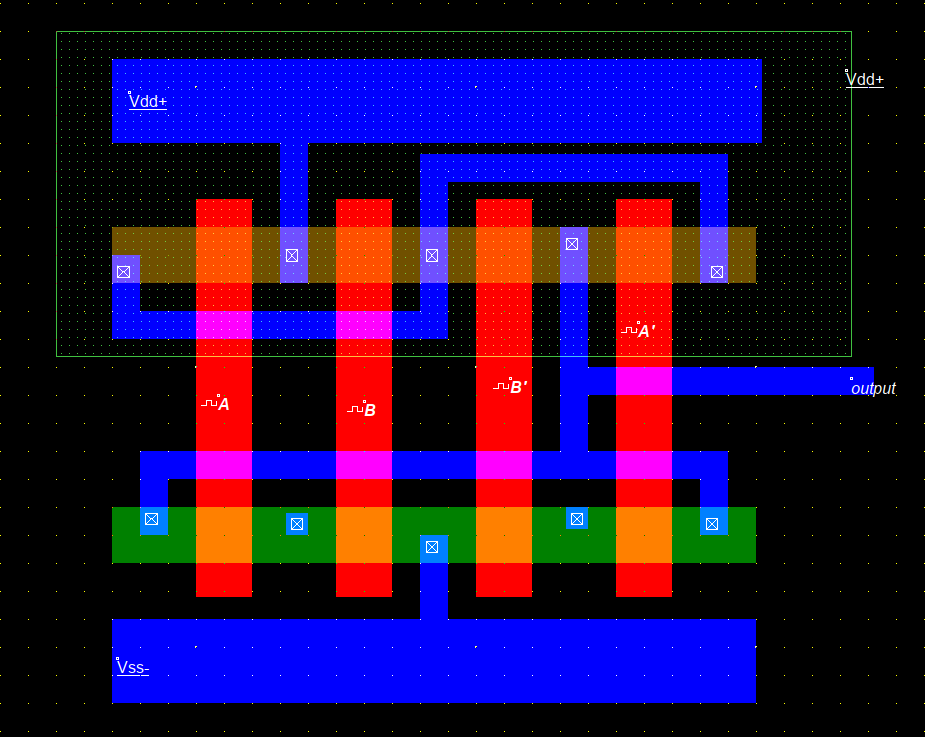
\includegraphics[width=0.7\textwidth]{Lab-06/XOR-Function-Stick-Diagram.png}
\caption{Stick Diagram of XOR Gate}
\end{figure}
\newpage
\subsection*{Output}
\begin{figure}[!h]
\centering
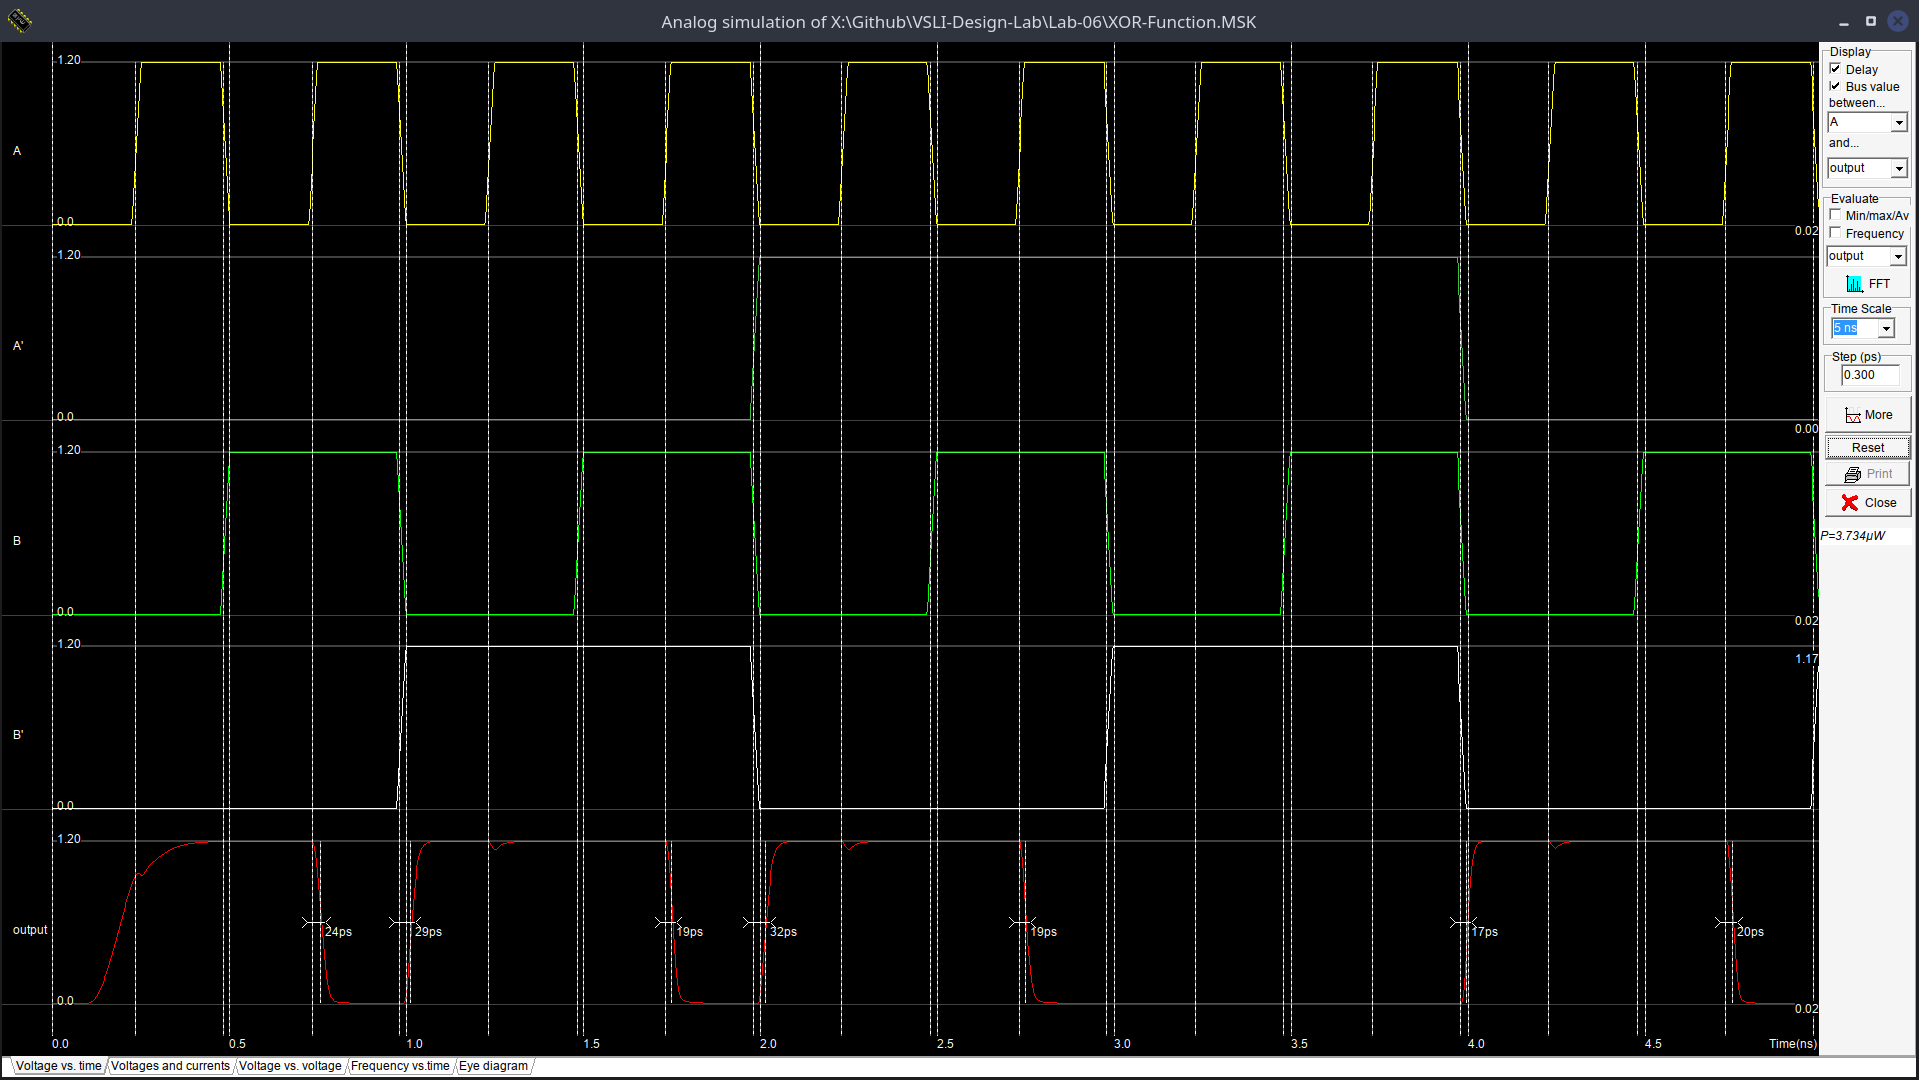
\includegraphics[width=1\textwidth]{Lab-06/XOR-Function-Output.png}
\caption{Output in Analog Simulation of XOR Gate}
\end{figure}

\subsection*{Observation}
From the implementation and simulation of the XOR gate stick diagram using Microwind2, it was observed that the circuit produces a logic HIGH output when the inputs are different and a logic LOW output when both inputs are the same. The output waveform obtained from the simulation matches the theoretical truth table of the XOR function.

The stick diagram correctly represents the CMOS structure using appropriate placement of polysilicon, diffusion, and metal layers. Proper alignment and interconnection of these layers ensured correct signal flow and circuit operation. The simulation results confirm that the designed layout accurately implements the XOR logic function.



\chapter*{\center Conclusion}
\addcontentsline{toc}{chapter}{Conclusion}
<Write Conclusion here>

\end{document}